\documentclass[12pt, a4paper, twoside]{report}
\usepackage[utf8]{inputenc}
\usepackage{blindtext}
\usepackage[margin=2cm]{geometry}
\usepackage{markdown}
\usepackage[hyperref]{xcolor}
\usepackage{setspace}
\usepackage{newpxtext}
\usepackage{newpxmath}
\usepackage[margin=1cm, labelfont=bf]{caption}
\usepackage{subcaption}
\usepackage{booktabs}
\usepackage{numprint}
\usepackage{inconsolata}
\usepackage{mathtools}

\usepackage{graphicx}
\linespread{1.5}
\usepackage{xspace}
\usepackage{tikz-feynman}

% Biblatex
\usepackage[sorting=none]{biblatex}
\bibliography{bibliography}

% Hyperlinks
\definecolor{blue1}{RGB}{50, 142, 237}
\definecolor{red1}{RGB}{239, 83, 138}
\definecolor{orange1}{RGB}{243,109,33}
%\usepackage[colorlinks=true, allcolors=blue1]{hyperref}
\usepackage[colorlinks=true, allcolors=orange1]{hyperref}
\usepackage{soul}
\usepackage{amsmath}
\usepackage{bm}
\usepackage{marginnote}
\usepackage{adjustbox}

\usepackage{sepfootnotes}

\usepackage[group-separator={,},separate-uncertainty=true]{siunitx}
\DeclareSIUnit\clight{\text{\ensuremath{c}}}

% Acronyms
\usepackage[acronym,nonumberlist]{glossaries}
\renewcommand*{\glstextformat}[1]{\textcolor{black}{#1}}
%\makeglossaries
\newacronym{COMET}{COMET}{Coherent Muon-to-Electron Conversion}

% Path of figures for each chapter
%\graphicspath{{introduction/}{chapter2/}{conclusion/}}

%
\newcommand{\diff}[2]{\frac{\textrm{d}{#1}}{\textrm{d}{#2}}}

% If table of contents goes too deep, we can limit depth.
%\setcounter{tocdepth}{0}

% Color scheme: https://coolors.co/0081a7-00afb9-fdfcdc-fed9b7-f07167

\begin{document}

% Title page
\thispagestyle{empty}
%\includegraphics[width=0.0\textwidth]{IMP_ML_1CS_4CP.eps}


\vspace*{\fill}

\begin{center}
    
    {\huge Sensitivity Estimates and\\[-0.2cm]
    Background Study toward the \\[-0.2cm]
    COMET Phase-I Experiment \par }%Conversion Search \par}

    \vspace{1cm}
    
    {\Large Matthias Dubouchet}

    \vspace{0.8cm}
    
{\large
High Energy Physics Group\\[-0.2cm]
Department of Physics\\[-0.2cm]
Imperial College London \par
}


    \vspace{1.5cm}
    \includegraphics[width=0.35\textwidth]{title_page_graphic.png}
    \vspace{1cm}
    
    {\large Submitted in partial fulfilment of the requirements\\for the degree
    of Doctor of Philosophy}
    
\end{center}

\vspace*{\fill}
\clearpage

% Blank page
\shipout\null

\pagenumbering{roman}

\chapter*{Abstract}

300 words max


\include{declaration}

\chapter*{Acknowledgements}



I acknowledge the important contributions from Noam Mouelle and Irene Andreou to
the model evaluation methods and results described in
Section~\ref{sec:quality_metrics}, and the fruitful discussions with Valentin Niess
about his original study of cosmic ray-induced backgrounds in COMET Phase-I and
his backward Monte Carlo simulation method.

\tableofcontents
\printglossary[type=\acronymtype]
\clearpage

\pagenumbering{arabic}

\chapter{Lepton Flavour in the Standard Model and Beyond}\label{chapter1}

% \begin{markdown}
% ---

% + Yoshi said: this is really an intro to CLFV searches for experts out of the
% field.

% + What's a muon?
% + What does the SM predict muons can/can't do
% + Historical context, motivation
%  + Why/how was the first CLFV experiment conducted?

% Sindrum II: what do they start with?
%  - Generation mixing in neutrino oscillations


% ---
% \end{markdown}

% v1
The Standard Model (SM) of particle physics is possibly the most successful
mathematical model of physical phenomena so far. It provides accurate
predictions for all observable interactions between known elementary particles.

% The very start of this chapter should introduce HEP concepts like the muon and
% what it is, how it relates to the SM, what is the SM.

% This thesis concerns itself with addressing some of the challenges faced in the
% simulation of particles within the experimental setup of the COMET experiment.

% However before we are able to dive into the main topics, it is necessary to
% discuss the purpose of the experiment, how it emerges from the current state of
% our knowledge of elementary particle physics, and the steps taken to get there.


% v0
% Explain the SM. Something like
% The Standard Model is the theory at the heart of modern particle physics. Built
% upon special relativity and quantum mechanics, it describes the interactions
% between elementary particles and allows physicists to predict the outcome of
% interactions and decays to a previously unattainable precision. Little evidence
% so far has been able to contradict the formulation of the Standard Model,
% despite many fundamental questions remaining unanswered, such as the nature of
% dark matter, the reason for the matter-antimatter asymmetry in the universe, or
% the existence of exactly three generations of leptons and quarks.


\section{Discovery of the muon}
The first traces of muons were observed around 1937 by three experiments
investigating the nature of cosmic ray-induced particle
showers~\cite{PhysRev.51.884, PhysRev.52.1198, PhysRev.52.1003}. 
In addition, one analysis was able to estimate the mass of the discovered
particle at 130 times that of the electron. 
In 1935, Yukawa predicted the existence of a particle with a similar mass whose role
was to carry the strong force and bind atomic nuclei
together~\cite{10.1143/PTPS.1.1}. Hence the muon and Yukawa's particle were
originally believed to be one and the same particle, and it was only when
Yukawa's meson (now called $\pi$, for primary) was observed decaying into a muon,
that the two particles were completely disambiguated~\cite{LATTES1947}.

It was the fact that the muon appeared as nothing but a heavy electron which
prompted Rabi to ask ``who ordered that?'' in response to its discovery. In
fact, the Standard Model still cannot give a satisfactory answer to this
question as it does not motivate the existence of three generations of
elementary particles. As far as the SM can explain, there is no fundamental reason
for the existence of distinct flavours.

\section{The muon in the Standard Model}
% 
The SM identifies the muon as the second-generation charged lepton, meaning it
is a fermion with identical quantum numbers (aside from flavour) as the electron
and tau lepton. The only way for a muon to decay in a vacuum is through the weak
force. The diagram for muon decay is shown in Fig.~\ref{fig:weak_decay}.


\begin{figure}
    \centering
    \feynmandiagram [layered layout, horizontal=a to b] {
        a [particle=\(\mu^{-}\)] -- [fermion] b -- [fermion] f1 [particle=\(\nu_{\mu}\)],
        b -- [boson, edge label'=\(W^{-}\)] c,
        c -- [anti fermion] f2 [particle=\(\overline \nu_{e}\)],
        c -- [fermion] f3 [particle=\(e^{-}\)],
    };
    \caption{Feynman diagram for the weak decay of the muon.}
    \label{fig:weak_decay}
\end{figure}

% mu -> e gamma
The process $\mu \rightarrow e + \gamma$ is in principle kinematically allowed
as well, and the SM contains no symmetry which would forbid such a flavour
change. However, it has never been observed experimentally. Since
1948~\cite{PhysRev.73.257}, searches for ${\mu \rightarrow e + \gamma}$ have
demonstrated that it does not occur at any observable rate: the current upper
limit on its branching ratio measured by the MEG experiment is
$10^{-13}$~\cite{mori2016final}.

In the quark sector, generations can mix via weak interactions: the
CKM matrix accurately describes how strongly each quark flavour couples
to the others. %~\cite{PhysRevLett.10.531, 10.1143/PTP.49.652}.
For leptons on the other hand, it is
only through neutrino oscillations, discovered by the Super-Kamiokande
experiment~\cite{PhysRevLett.81.1562}, that flavours have been observed to mix. 
Flavour-changing neutrino oscillations allow a new channel for ${\mu \rightarrow
e + \gamma}$, shown in Fig.~\ref{fig:mu_e_nu_osc}. However, the branching ratio
calculated for this process using the upper limit on neutrino masses is given
by:
$$
\mathcal{BR}(\mu \rightarrow e + \gamma) = \frac{3\alpha}{32\pi} \left|\ \sum_{i=2, 3} U^*_{\mu i} U_{e i} 
\frac{\Delta m^2_{i1}}{M^2_W}  \ \right| ^2 \approx 10^{-54},
$$
where $U$ is the PMNS matrix, $\Delta m^2_{ij}$ is the mass-squared difference between the
$i$-th and $j$-th neutrino mass eigenstates, and $M_W$ is the $W$-boson
mass~\cite{BERNSTEIN201327}.
Any evidence that the ${\mu \rightarrow e + \gamma}$ process occurs at a higher
rate than this would indicate that another channel involving charged lepton
flavour violation (CLFV) is responsible.

\begin{figure}
    \centering
    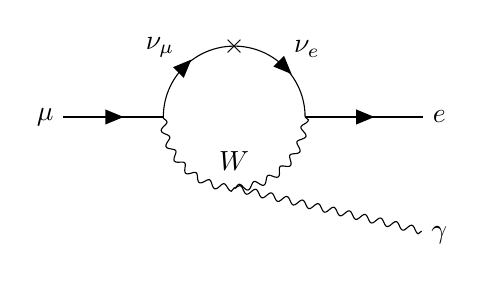
\begin{tikzpicture}
    \begin{feynman}
    \vertex (a) {\(\mu\)};
    \vertex [right=1.5cm of a] (b);
    \vertex [right=1.8cm of b] (c);
    \vertex [right=1.5cm of c] (d) {\(e\)};
    
    \vertex at ($(b)!0.5!(c) + (0, 0.9cm)$) (n);
    \vertex at ($(b)!0.5!(c) + (0, -0.9cm)$) (w);
    \vertex [above=0.1cm of w] (wn) {\(W\)};
    \vertex [below=1.5cm of d] (g) {\(\gamma\)};
    
    \diagram* {
    (a) -- [fermion] (b)
    -- [fermion, quarter left, edge label=\(\nu_\mu\)] (n)
    -- [fermion, quarter left, edge label=\(\nu_e\)] (c),
    (b) -- [boson, quarter right] (w)
    -- [boson, quarter right] (c),
    (c) -- [fermion] (d),
    (w) -- [boson] (g),
    };
    
    \draw (n) -- (n) node {\(\times\)};
    
    \end{feynman}
    \end{tikzpicture}
    \caption{
        Feynman diagram for $\mu \rightarrow e + \gamma$ via
        flavour oscillation of a virtual neutrino.
    }
    \label{fig:mu_e_nu_osc}
\end{figure}



In the presence of matter, there are additional processes which could be
investigated to find charged lepton flavour violation (CLFV), as shown in Fig.


% Allowed and forbidden decays

% g-2 measurement
\cite{PhysRevLett.126.141801} % g-2

% Is lhc-b related here? Lepton univ?
\cite{lhcbcollaboration2021test} % lhc-b R_K




\section{Charged lepton flavour violation}
Quark generations are known to mix (CMK).
Neutral leptons (neutrinos) are known to mix (PMNS, osc).
Charged leptons have never been seen to mix. Why?

\begin{figure}
    \centering
    \includegraphics{chapter1/clfv_upper_limit_v2.pdf}
    \caption{90\%-confidence upper limit on the branching ratio of three charged lepton flavour-violating processes over time. The past data points were tabulated in~\cite{BERNSTEIN201327}. Future data points are the expected sensitivities quoted in the MEG II~\cite{Baldini2018}, Mu3e~\cite{ARNDT2021165679}, COMET Phase-I~\cite{the_comet_collaboration_comet_2020} and Mu2e~\cite{bartoszek2015mu2e} design reports.}
    \label{fig:clfv_upper_limit}
\end{figure}

%The search for Lepton Flavour Violation started in 19XX with John Doe's experiment~\cite{doe}.



%See Chapter~\ref{chapter2}, read~\cite{goodfellow_generative_2014}.\\
%The smooth boi can be seen on Fig.~\ref{subfig:smooth_boi}, and the outlined boi on %Fig.~\ref{subfig:smooth_boi}. The whole figure is Fig.~\ref{fig:my_label}.
%
%A derivative:
%$$\diff{x}{y} = 2\pi x y$$
%Insane!
%
%And here we typeset COMET in smallcaps: \COMET. This \acrshort{COMET} is an \emph{acronym}. %You can click it to see what it means.
%
%\begin{figure}
%    \centering
%    \subfloat[A smooth boi]{
%    \includegraphics[width=0.5\textwidth]{viewer_smooth.png}
%    \label{subfig:smooth_boi}
%    }
%    \subfloat[An outlined boi]{
%    \includegraphics[width=0.5\textwidth]{viewer_outline2.png}
%    \label{subfig:outlined_boi}
%    }
%    \caption{Phase-I cutaway geometries.}
%    \label{fig:my_label}
%\end{figure}
%
%Here we cite the COMET TDR~\cite{the_comet_collaboration_comet_2020} and the upper limit on %the branching ratio of $\mu^- + \textrm{Al} \rightarrow e^- + \textrm{Al}$, $7\times %10^{-13}$, by the SINDRUM-II experiment~\cite{Bertl:2006up}.

\chapter{The COMET experiment}\label{chapter2}

\begin{markdown}
---

- Description of the COMET experiment's goal, design with nice illustrations
    + *Reference next chapter for geometry renderings*
    + Signal and background:
        + mu-e conv signal description
        + **List of background sources**
+ CyDet:
    + For simulation section, need to explain how CDC and CTH work, and how combined they enable mu--e conv measurement
    - Detailed description of the CDC, which is crucial for the GAN section.
     - Stereo angles
+ Phase alpha

- References: TDR, SINDRUM II, 

---

+ Requirements: high sensitivity to signal, efficient rejection of backgrounds
 + -> Need intense muon beam, pulsed, and detector design must avoid backgrounds
+ TIMING of signal (muon lifetime)
+ Proton beam energy: why 8 Gev -> antiproton production
+ Intensity: beam current, beam power, POTs per second
+ Send backward-going secondaries to detector, discard the main part of secondaries (forward-going)
+ Curved solenoid + dipole field (by tilting coils, see Krikler)
+ Stopping target -> why Al
+ Bunch structure, extinction
+ Phase-I detectors: StrECAL and CyDet

---
\end{markdown}

COMET (COherent Muon-to-Electron Transition) is a muon-beam experiment aiming to
observe the muon-to-electron conversion process, or at least to constrain its
branching ratio to an unprecedented upper limit. Currently being built at the
J-PARC facility in Tokai, Japan, its physics program will be run in a two-stage
approach, Phase-I and Phase-II. These two phases are expected to improve our
sensitivity to the conversion signal by factors of 100 and \num{10000},
respectively, with respect to the current world-leading measurement conducted at
the SINDRUM II experiment~\cite{Bertl:2006up}.




The design of the COMET experiment is heavily angled toward suppressing
backgrounds to the $\mu$--$e$ conversion signal. Understanding the background
sources and their properties is key in making sense of the experimental design.

\section{The COMET beam}\label{sec:COMET_beam}

\section{Experimental backgrounds}\label{sec:backgrounds}

% The choice of target material directly influences how frequently high-energy
% electrons will be produced by these processes, and hence contributes in
% setting the maximum experimental sensitivity.

% This should go into the COMET section as these are specific to COMET and/or
% specifically addressed by the COMET design.
% Background events can be classified into three categories: intrinsic,
% beam-related, and cosmic ray-induced.

% Beam-related backgrounds come from impurities in the high-intensity muon beam.
% The specifics of the COMET beam and how these backgrounds are alleviated is
% discussed in Section~\ref{sec:COMET_beam}.

% Cosmic rays typically produce muons with a wide range of energies in the
% atmosphere which 
\chapter{Software and Simulation}
\label{chapter3}

\newcommand{\SimG}{\texttt{SimG4}\xspace}
\newcommand{\oaEvent}{\texttt{oaEvent}\xspace}
\newcommand{\Geant}{{\sc Geant4}\xspace}

% \begin{markdown}
% ---

% + Introduce ICEDUST, the COMET software suite
%     + Describe whole, then individual parts
%     + oaEvent
 
% + Important part of the software is the set of simulation tools
%     + COMET geometries
%     + Physics, "physics list"?
%     + Show signal event display
%     + SDs, CDC hit representation
%     + RooTracker files
%     + Proton beam input?
%     + Hit merging and bunch simulation
%     + Large-scale production, MC5: Sampling world, example of results?
    
    
% + Version control
% + Continuous integration (+ CD, docker containers)
    
% + Mention miscellanous contributions:
%     + Beginner's tutorial (installation, simulation, analysis)
%     + Move from CMT to CMake and from ROOT5 to ROOT6
%     + Memory leaks and errors
%     + Backward MC: perhaps just ref chapter

% + Animated visualisation of CyDet activity

% ---
% \end{markdown}

Experiments in high energy physics are commonly accompanied by the development
of a set of software tools to help in manipulating and analysing experimental
data. Simulations are used extensively to optimise experimental designs and
prepare for the collection of real data while the physical instruments ---
detectors, magnets, readout electronics and data acquisition systems --- are
being manufactured and assembled.

\section{The ICEDUST Software Suite}
The COMET Collaboration develops a suite of software packages named ICEDUST
(Integrated COMET Experimental Data User Software Toolkit) to satisfy the
offline data-processing requirements of the experiment. Originally forked in
2013 from the software written for T2K's near detector system ND280, ICEDUST
supports the needs of the COMET experiment with regard to simulation, on-disk
data format, calibration, reconstruction and analysis.
Figure~\ref{fig:icedust_schematic} shows the flow of real and simulated data
within the ICEDUST framework, and lists the names of the key packages for each
step.


\begin{figure}
    \centering
    \includegraphics[width=0.9\textwidth]{chapter3/ICEDUST_vertical.drawio.pdf}
    \caption{Data flow in the ICEDUST framework. The colour of arrows represents
        the data format. By design, simulated detector data and real data share
        a common format such that they can be processed identically by the
        calibration, reconstruction and analysis stages.}
    \label{fig:icedust_schematic}
    \vspace{1.2cm}
    \includegraphics[width=0.6\textwidth]{chapter3/oaEvent.drawio.pdf}
    \caption{Layout of \oaEvent files which contain MC or real data. Blue arrows
    in Figure~\ref{fig:icedust_schematic} indicate steps of the data flow where
    data is stored in this format on disk.}
    \label{fig:oaEvent}
\end{figure}

\subsection{Data format}
A key design principle of ICEDUST is to define a common format adopted by both real and simulated data, such that the pipeline of calibration, reconstruction and analysis can be thoroughly tested with only simulation data, in advance of the data acquisition stage. 
This offline data format is called \oaEvent. Based on the ROOT~\cite{BRUN199781} serialisation system, \oaEvent defines a file format where data is laid out as a sequence of events, shown schematically in Figure~\ref{fig:oaEvent}. Each event object contains an arborescence of data containers, each of which holds an array of some given data type (e.g.\ detector hits, calibrated energy deposits, reconstructed tracks, etc.).

From Phase-I onward, data will be collected using the MIDAS data acquisition system, hence the online on-disk format is based on MIDAS data banks. ICEDUST provides a direct translation from this format to \oaEvent via the \texttt{oaRawEvent} and \texttt{oaUnpack} packages. Once translated, the data can flow through the calibration, reconstruction and analysis stages.

%Prior to calibration, the resulting data will typically represent uncalibrated, digitised detector hits or waveforms. 

%The term ``event'' here is purposefully abstract, as the information held in each event can vary. In simulations, an event can describe the outcome of a single proton-on-target (POT) collision, or the outcome of a full proton bunch ($16\times10^6$ POT). 
%In data-taking runs, the definition of event will typically be dictated by the data acquisition system.  % So?



%Each event is its own hierarchical ``directory'', where data containers can be stored and retrieved by name. The containers themselves are variable-length arrays of arbitrary data types---defined as C++ classes---where objects of the same type can be aggregated.


%The calibration step uses pre-established calibration databases for each sub-detector to convert the digitised information into physical information such as the energy deposit and time that constitute hits. The reconstruction algorithms process hits to find tracks and filter out background, to pass that information down to the final analysis stage.

\subsection{Simulation pipeline}
Simulations of the COMET experiment can be split into four steps:
\begin{enumerate}
    \item {\bf Event generation} takes place at the level of individual protons. A proton beam profile is drawn ahead of time using a specialised Turtle~\cite{Carey1974DecayT} simulation of the beamline. The position and momentum of the protons are histogrammed at a short distance ahead of the pion-production target. Protons are sampled from the resulting distribution to generate events, and the outcome from each primary proton is referred to as a proton-on-target (POT) event.
    \item {\bf Particle tracking} is the step-by-step propagation of particles through the geometry and electromagnetic fields of the experimental setup. The primary proton will usually produce many secondary particles in the collision, some of which might propagate to the detector region. Simulated energy deposits in the active detector volumes are recorded for the detector response simulation stage.
    \item {\bf Event bunching} allows us to model the simultaneous arrival of a proton bunch into the setup. In the real beamline, millions of protons are bunched into a short \SI{{\sim} 100}{\ns} time interval, and two consecutive bunches are separated by about \SI{1.2}{\micro\second}. In order to simulate this time structure, a time offset is applied to each POT event, after which the events are merged into bunches. Following this, individual bunch events can be further merged into \emph{bunch trains} to obtain an entire sequence and account for potential pileup.
    \item {\bf Detector response simulation} translates the true energy deposits simulated in the particle tracking stage into detector-specific hits. It takes into account the way in which charge or light is collected by the detector, and can apply smearing to the observed energy and timing. This step effectively reverses the calibration process by transforming energy deposits into uncalibrated, digitised hits and waveforms.
\end{enumerate}
% ^ OK
Once all four stages of the simulation pipeline are complete, the result should closely resemble real data post-translation from MIDAS to \oaEvent. This implies that it should be able to naturally flow through the calibration, reconstruction and analysis stages. At each stage, the information may be compared with the truth information available from the particle tracking stage in order to refine each process. This exercise should also outline the performance of the offline data-processing pipeline and hence provide an estimate of the computational requirements of the experiment.


\subsection{Intermediate simulation file format}
\label{subsec:RT}
The \texttt{oaRooTracker} package defines another ROOT-based file format used by the simulation to save and retrieve particle states. The typical use case is for a simulation to record particles that have reached a key geometrical element (e.g.\ the detector region) to build up a sample of interesting events. The saved particle states can then be used as input to subsequent simulations, easing the need for a full simulation run every time a change is made to the geometry or physics models.

In addition, from a large enough sample of particles recorded at some key volume boundary, the flux distribution of inbound particles can be estimated. Events can then be sampled from this distribution to increase the statistics inside the volume of interest. 

% RooTracker files
%The simulation software provides utility to record particles that reach certain key points in the geometry, such as the transport solenoid or the detector region. Virtual monitors are volumes that can be placed in the geometry to record the passage of particles, in the form of virtual hits or into a separate file. The file format used to save particle states is called \texttt{RooTracker}. It stores the kinematics of simulated particles and can thus be used as input to another simulation run. % and?

\section{Monte Carlo simulation in ICEDUST}
\label{sec:mc_sim}
Monte Carlo (MC) simulation is the process through which hypothetical particles are realistically propagated through an experimental setup, with the aim of evaluating the experiment's performance and to prepare for its realisation. Currently in COMET, MC simulations are heavily used to further optimise the experiment's design and to develop reconstruction and analysis algorithms.

Monte Carlo simulation in high energy physics can be described as the stepwise propagation (tracking) of particles through matter and electromagnetic fields. Starting from initial conditions of position and momentum, a particle advances in space and time according to the laws of relativistic kinematics. It can change velocity or direction, and produce secondary particles via interactions with the local medium and field. The tracking of a particle ends when it decays, gets absorbed by some material, or exits the simulation space.

Interactions and decays occur stochastically according to measured cross-sections and lifetimes. Depending on the type of interaction, secondary particles may be emitted. In this case, the position and momentum of secondaries are stored in memory until the tracking of the primary particle is finished. The list of secondaries is then iterated through, propagating each one in turn. Since secondaries may produce their own secondaries, this process continues recursively until all products of the original primary particle have been accounted for.
% ^OK

In ICEDUST, particle tracking, event bunching and detector response simulation are handled in separate packages.
Particle tracking can be performed using four different engines: Geant4~\cite{AGOSTINELLI2003250}, FLUKA~\cite{FLUKA}, MARS15~\cite{MARS15} and PHITS~\cite{PHITS}. The corresponding ICEDUST packages are \SimG, \texttt{SimFLUKA}, \texttt{SimMARS}, and \texttt{SimPHITS}, respectively.
Event bunching is handled by the \texttt{SimHitMerger} package, and \texttt{SimDetectorResponse} performs detector response simulation.

\subsection{Geometry}
The \SimG package contains the most detailed and up-to-date definitions of the COMET simulation geometries.
The various components that make up a simulation world are defined with constructive solid geometry, using the standard \Geant geometry classes. In addition, \SimG extends the \Geant macro language to allow geometrical parameters to be defined in macro files. The position, dimensions, and material of every volume can thus be specified at run-time rather than compile-time. A custom parser attached to every volume allows interdependencies between components and supports looping, for instance to position identical elements in a regular pattern.

Once the simulation geometry is assembled, it is also translated into the ROOT \texttt{TGeo} representation, which simplifies its visualisation and its storage on disk as metadata inside \oaEvent files. This representation can furthermore be interpreted by the MARS15 tracking software, which simplifies the process of running comparative simulations.

%Once the whole geometry is assembled, it is translated into an equivalent ROOT representation that will be stored into the output file for book-keeping. This copy can also be rendered more readily by the 3D utility classes of the ROOT package. % Link to DisplayCore? !! REMOVED --> out of scope of section?


The \SimG package includes geometries for the Phase-$\alpha$, Phase-I (CyDet and StrawECAL configurations), and Phase-II setups. Over time, these simulation worlds are refined by developers to better reflect the exact configuration of the experiment. 
Figure~\ref{fig:comet_geometries} shows the simulation geometries for the two conversion-searching COMET designs.

\begin{figure}
    \centering
    \captionsetup[subfigure]{justification=centering}
    % To make this figure: thin wireframes, white background
    % Plane clipping at y=10
    % zoom all the way out and move the camera forward (right-click)
    % so the perspective approaches an isometric view.
    \noindent\makebox[\linewidth][c]{
    \begin{subfigure}[t]{0.57\textwidth}
        \centering
        \includegraphics[width=0.95\textwidth]{chapter3/geometries_Phase-I_iso_cropless_huesat_croppedleft.png}
        \caption{Phase-I in the CyDet configuration.}
    \end{subfigure}
    \hfill
    \begin{subfigure}[t]{0.57\textwidth}
        \centering
        \includegraphics[width=0.95\textwidth]{chapter3/geometries_Phase-II_iso_huesat_human.png}
        \caption{Phase-II.}
    \end{subfigure}}
    
    \caption{Cutaway views of the simulation geometries implemented in \SimG and visualised with \texttt{DisplayCore}. The experiment hall is also modelled in the simulation but was hidden here for clarity.}
    \label{fig:comet_geometries}
\end{figure}

% vvvv Moved to first section
% % Event generation 
% \section{Event generation and bunch structure}
% Protons are sampled from a beam profile histogram at a distance of \SI{70}{\cm} upstream of the target. The histogram is generated via a Turtle~\cite{Carey1974DecayT} simulation of the proton beamline.

% In the simulation, a single proton is sampled from the beam histogram for each event, which differs from the real situation in that the actual beam is arranged into bunches, each containing about 16 million protons. Hence we assume that proton collisions in a bunch are independent of each other, and we merge POT events into bunch events by overlaying the produced trajectories and hits. This task is handled by the \texttt{SimHitMerger} program after \SimG has finished simulating single-proton events. The time structure of the proton bunch is modelled as a square wave with a width of \SI{100}{\ns}. To simulate this structure, a time shift is sampled uniformly between -50 and \SI{50}{\ns} for each POT event and applied to every trajectory and hit.

% \hl{Refer to, or show a time structure diagram}
% ----------

\subsection{Physics}
The COMET experiment involves many physical processes to go from the initial proton collision to backgrounds in the detector.
The MC simulation must faithfully account for any process which could lead to backgrounds if we are to realistically estimate the experiment's sensitivity. 
Hence, the \SimG simulation associates standard \Geant hadronic and electromagnetic physics lists with custom logic for nuclear muon capture and muon decay-in-orbit.

To model hadronic interactions, \SimG uses the \texttt{QGSP\_BERT\_HP} reference physics list as the default. In this model, hadron-nucleus interactions between the \SI{8}{\GeV} proton beam and the pion-production target are handled by the Bertini Cascade model~\cite{WRIGHT2015175}.

Muons at rest receive special treatment in \SimG due to their important
contribution toward the background rate. The default energy spectrum of
electrons from muon decay-in-orbit is replaced by the numerical evaluation
of~\cite{czarnecki}, which includes the effect of nuclear recoil and thus allows
electron energies up to \SI{104.973}{\MeV}. In addition, the nuclear muon
capture (NMC) model is replaced to adhere to the results of the AlCap
experiment~\cite{PhysRevC.105.035501} which measured the energy spectrum of
protons emitted after NMC in aluminium.




\subsection{Signal simulation}
By default, the list of physical processes considered by \SimG includes only SM-allowed interactions and decays, and hence does not include $\mu$--$e$ conversion. In order to simulate signal events, one can manually produce conversion electrons out of the muons stopped inside the stopping target.

From the normal beam simulation, one can estimate the spatial distribution of muons stopped in the stopping target and subsequently sample conversion electrons from it. In sensitivity studies, signal events are commonly overlaid onto a pure background sample in order to evaluate the signal acceptance and background rejection efficiencies of the hit filtering and track finding routines. % Accurate?

\begin{figure}
    \centering
    \captionsetup[subfigure]{justification=centering}
    \begin{subfigure}[t]{0.43\textwidth}
    \centering
    \includegraphics[width=0.95\textwidth]{chapter3/signal_event_display_crop_axes.pdf}
    \caption{Event shown in \texttt{DisplayCore}, the 3D event display.}
    \end{subfigure}
    \hfill
    \begin{subfigure}[t]{0.48\textwidth}
    \centering
    \includegraphics[width=0.95\textwidth]{chapter3/cydet_signal_track_v2.pdf}
    \caption{Event as seen by the CDC and CTH detectors.}
    \end{subfigure}
    
    \caption{Example of a simulated signal trajectory in the CyDet system. This particular event triggers the CTH and would be considered as an ideal candidate of a $\mu$--$e$ conversion signal.}
    \label{fig:signal_event}
\end{figure}

Figure~\ref{fig:signal_event} shows a simulated conversion electron emerging from the stopping target, depositing energy inside the CDC gas, to eventually trigger the CTH by hitting four adjacent counters. 

\subsection{Representation of simulated CDC hits}
\label{subsec:SD}
% Sensitive detectors, truth-hit representation
As a particle passes through a material, it tends to lose energy to the medium, e.g. through inelastic scattering or ionisation. 
In MC simulations, simulated energy deposits must be recorded inside active detector elements in order for us to determine the response of the detector and readout systems to the passage of the particle.

Detector elements in a \Geant simulation are defined as ``sensitive volumes'', and energy deposits of incoming particles are accumulated and recorded as ``hits''. 
The way in which hits are instantiated is typically dependent on the type of detector, because of differing granularities between e.g.\ a plastic scintillator and a drift chamber. A higher-granularity detector type requires finer-detailed information, hence more hit instances along the trajectory.

In \SimG, the data type associated with CDC hits is called \texttt{IG4HitGas}. When \Geant reports an energy deposit inside the CDC, an instance of that class is created. If a particle makes multiple steps in a CDC cell, the deposit from each step is accumulated into the same hit instance, such that only one instance per particle per cell may exist. If a particle enters the same cell multiple times, one hit instance is created per entry.
This is shown in Figure~\ref{fig:sim_cdc_hits}, where the position and granularity of \texttt{IG4HitGas} instances is drawn along an electron's trajectory in the CDC.


% In early 2019, ICEDUST developers agreed to change the definition of hits inside the CDC gas volume in order to more accurately portray the energy deposit information in that detector. Along that process, I came to be thoroughly involved in the testing and refinement of this new CDC hit representation, named \texttt{IG4HitGas}. 

% A hit representation is formulated as a C++ class which holds the hit's data. It must be coupled to a sensitive detector class, whose role is to receive information from \Geant's particle tracking system and accumulate it into instances of the hit class. For example, the sensitive detector class for a calorimeter might produce hits containing the total energy deposited for each inbound particle as well as a timestamp.

\begin{figure}
    \centering
    \includegraphics[width=0.5\textwidth]{chapter3/hit_instances_blur_crop.png}
    \caption{Hits, shown as red dots, produced by the CDC's sensitive detector class when a particle deposits charge inside the gas. One instance of \texttt{IG4HitGas} is created every time the particle traverses a CDC cell, i.e.\ roughly every \SI{16}{mm}.}
    \label{fig:sim_cdc_hits}
\end{figure}


This new hit class and the associated algorithms were introduced to \SimG in 2019. This hit representation is designed toward gaseous detectors, hence it also applies to the Straw-Tube Tracker of Phase-I and Phase-II. 
Because of the relatively low density of hit instances along a trajectory, important details of the true energy deposition pattern may be lost. Hence \SimG implements a run-time option to store \emph{auxiliary points} inside each hit instance, which provide a more fine-grained description of the particle's steps inside the cell.

% The \texttt{IG4HitGas} class was designed to condense and record energy loss information inside gaseous ionisation detectors in \SimG (e.g. the CDC and Straw-Tube Tracker). Every energy deposit made by a particle inside the same CDC cell is accumulated into a single instance of the class, such that only one hit per cell per particle may exist. While this saves memory and disk space, it limits the amount of detail that can be stored. The recorded information allows for basic detector response simulation, but if more detail is required one can tune the \SimG simulation to store finer details inside each \texttt{IG4HitGas} instance.



\section{Large-scale simulation: MC5}
\label{sec:mc5}
The 5th large-scale production of simulation data, MC5, was run in 2020 using computing facilities at the French National Institute of Nuclear and Particle Physics Computing Centre (CC-IN2P3) in Lyon, France.
Using \numprint{2000} concurrent machines over the course of a few weeks, the outcomes of 1 billion proton-on-target (POT) collisions were simulated with \SimG in the CyDet configuration of COMET Phase-I.

\subsubsection{Software}
Leading up to the MC5 production, several aspects of the software were changed or updated in comparison with the previous large-scale production:
\begin{itemize}
    \item The CMake build configuration system was introduced to replace the legacy CMT system. 
    \item The external ROOT software, upon which the \oaEvent data format depends, was updated from major version 5 to 6.
    \item The CyDet geometry received multiple updates to make it as faithful as possible to the design, adding detailed elements such as readout boards and fixing errors in the positioning of CDC wires. 
    \item As discussed in Section~\ref{subsec:SD}, the treatment of energy deposits in the CDC was also changed to the \texttt{IG4HitGas} representation.
    \item All memory-related problems identified by \texttt{valgrind} at the time were resolved to bring the simulation software into a production-ready state.
\end{itemize}

\subsubsection{Run configuration}

\begin{figure}
    \centering
    \includegraphics[width=0.6\textwidth]{chapter3/sampling_plane_illu_ink.pdf}
    \caption{
        Top-down cutaway view of the running configuration for MC5,
        showing $1.6\times 10^5$ overlaid events (1\% of a bunch). The orange
        line shows the sampling boundary where particles that cross into the
        detector region via the beamline or wall are recorded. Only
        charged-particle trajectories are shown for clarity.
    }
    \label{fig:Phase-I Sampling World}
\end{figure}



The simulation was split into two stages by dividing the world along a boundary
which effectively separates the pion-production section and transport solenoid
(upstream) from the detector region (downstream), as shown in
Figure~\ref{fig:Phase-I Sampling World}. The boundary is set up to record the
position and momentum of particles which enter the detector region. Most
particles will enter via the beamline, but a small fraction (mostly neutrons)
also penetrates through the wall, floor and ceiling. In the upstream run, only
particles that enter the detector region are saved to disk, along with their
ancestors. Upon doing so, their position and momentum is recorded to an
\texttt{oaRooTracker} file (see Section~\ref{subsec:RT}) which is used as input for the
downstream simulation.

This way to proceed means that the upstream simulation is unaffected by the disposition of the detector region, hence one can perform the upstream run once and use the results to seed multiple downstream configurations, e.g.\ changing the detector geometry (e.g.\ between CyDet and the StrawECAL) or magnetic field. Since most of the simulation time is spent in the pion-production section, this gives a flexible way to produce high-statistics MC datasets in multiple experimental configurations.
%Another benefit is that it allows for re-seeding of the downstream run, whereby each event retains the same initial conditions but uses several different seedings of the random number generator, yielding a more diverse dataset at the cost of potentially biasing the sample.
% ^ Off-topic?

\subsubsection{Outcome}
The data produced with MC5 has a total disk size of \SI{13}{TB} and is archived on the tape storage system at CC-IN2P3. The sample size of $10^9$ POT events represents 62 unique beam bunches when merged, or the equivalent of $~\SI{0.1}{\ms}$ of data acquisition in Phase-I.

\section{Animated CyDet event display}
In order to visualise events in the CyDet system, I developed a tool to display hit data from MC simulations as animations, visually similar to a slow-motion online monitor of the detector. Figure~\ref{fig:animation} shows a series of frames from one such animation involving a $\mu$--$e$ conversion electron.

\begin{figure}
    \centering
    
    \captionsetup[subfigure]{justification=centering}
    \begin{subfigure}[t]{0.49\textwidth}
    \centering
    \includegraphics[width=0.95\textwidth]{chapter3/frame_005.png}
    \caption{$t=\SI{0}{ns}$. Ignoring pileup and cosmics, the detector is clear of hits before the POT collision.}
    \end{subfigure}
    \hfill
    \begin{subfigure}[t]{0.49\textwidth}
    \centering
    \includegraphics[width=0.95\textwidth]{chapter3/frame_036.png}  
    \caption{$t=\SI{155}{ns}$: many tracks occupy the detector soon after the beam flash.}
    \end{subfigure}
    
    \vspace{0.3cm}
    
    \begin{subfigure}[t]{0.49\textwidth}
    \centering
    \includegraphics[width=\textwidth]{chapter3/frame_067.png}
    \caption{$t=\SI{310}{ns}$: the hit rate decreases significantly once the beam flash has ended.}
    \end{subfigure}
    \hfill
    \begin{subfigure}[t]{0.49\textwidth}
    \centering
    \includegraphics[width=\textwidth]{chapter3/frame_192.png}
    \caption{$t=\SI{815}{ns}$: a conversion electron appears in the CDC and triggers the CTH.}
    \label{fig:animation:conv}
    \end{subfigure}
    
    \caption{Still frames of an animation rendered by the visualisation tool. The event shown outlines how a conversion electron would be seen by the CyDet system among background hits.}
    \label{fig:animation}
\end{figure}


% Visual features
The produced animations show the CyDet system under two projections such that particle trajectories can be visualised in all three dimensions, over time. The left-hand side of the display shows the projection in the readout plane, with the CDC on the outside and the CTH counters on the inside, while the right-hand side shows an orthogonal view with the same vertical axis.
In the centre of the left-hand pane, a histogram shows the rate of hits over the event's duration and a cursor indicates the current time in the simulation.

Each animation shows one bunch event unfolding over one cycle, i.e.\ \SI{1170}{\ns} from the collision of one bunch until the arrival of the next one. Time is slowed down by a factor of ${\sim}10^{-7}$ such that the event unfolds over 10 real seconds.

In the CDC, the true position of every hit is drawn as a circle with a radius proportional to the amount of energy deposited. Colour indicates hits produced by the same particle such that tracks can be disambiguated.

The CTH counters flash only in the case of a fourfold coincidence i.e.\ if four adjacent counters are struck within a \SI{10}{\ns} window.
Fourfold coincidences are most often caused accidentally by multiple particles, but occasionally a single track will hit four counters. In these occurrences, the track is emphasised in the animation and the particle type is displayed, as can be seen in Figure~\ref{fig:animation:conv}.

Hits in the CDC and CTH fade out over time such that the display does not become cluttered, but the fading rate is not representative of the actual time resolution of the sub-detectors.

% Implementation details
The animation rendering tool is written in Python. The code includes an algorithm for finding fourfold coincidences among CTH hits. To draw the frames, it relies on the \texttt{matplotlib} package. Once the individual frames have been rendered, a \texttt{bash} script runs \texttt{ffmpeg} to assemble them into a video format, such as \texttt{webm}, \texttt{gif} or \texttt{mp4}.


\section{Version control and continuous integration}

The source code of the ICEDUST software project is version-controlled using Git. A shared repository is hosted on the Gitlab instance of the IN2P3, where developers collaborate on building up and improving the code base. The repository contains a full history of the code, an issue tracker, and a set of wiki pages documenting the software. 

Additions and changes are submitted to the central repository through merge
requests from the developers. When submitting a merge request, changes to the
code are typically reviewed by another developer or maintainer who verifies that
no new bugs are introduced into the main branch. To further reduce the
likelihood of new issues appearing, the ICEDUST repository makes use of Gitlab's
continuous integration system.

Every time new code enters the main branch, the whole code base goes through a
three-step pipeline. The first step compiles the code and builds a new version
of every binary. The second step runs custom unit tests and validations using
this new build. Each unit test typically verifies that a single functionality
works as intended in an isolated environment, while validations can run multiple
pieces of the software and ensure that the results are consistent between one
revision of ICEDUST and the next.

If the building, unit testing and validation stages all pass, the pipeline moves to the final deployment step where the new binaries are assembled into a Docker image which is published to the repository's container registry. Users who wish to use the compiled software as-is can download this image and run it via Docker or Singularity.
If any of the pipeline steps reports a failure, the developer submitting the merge request is notified and full logs are provided to identify the issue. A merge request is usually only accepted once the code has been reviewed and if the pipeline finishes successfully.


\chapter[Data Augmentation with Generative Adversarial
Networks]{Data Augmentation with \\ Generative Adversarial
Networks}
% \begin{markdown}
% ---

% - We are coming from the simulation chapter, so:
% - Problem description: 
%  - We would like to produce larger amounts of simulation data, e.g. for a mock
%    dataset in preparation for data-taking
%  - But we have limited capability to produce MC data with simulation. The main
%    bottleneck is in the pion-production section's hadronic interactions. Is
%    there a faster way?
%   - The topic of this chapter is to consider the application of
%     machine-learning methods in the fabrication of fake Monte Carlo data.


% - Creation of dataset from Monte Carlo simulation
%   - Hit pattern characterisation
%   - Reconstructible vs noise-like classification
% - GAN theory [Goodfellow, WGAN, WGAN-GP]
%  - Pre-processing
% - GAN design, basic architecture, softmax for classes [WGAN-GP]
% - GAN extensions, embedding? analogy with text?

% ---
% \end{markdown}

% Need to wrap the start of this chapter into a compelling narrative:
% 1. MC allows us to see possible patterns in detector sys e.g., in CDC,
%    high-mom tracks produce structured hits whereas low-mom make small
%    localised hit clusters --> Draw figures
% 2. For an exercise such as a mock-data challenge (explain term), traditional
%    MC is not efficient enough to produce the dataset.
%  + Think about: why do we want mock data? Why is the standard sensitivity
%    estimation process not sufficient?
%    - Perhaps the extrapolation factor. Considering efficiencies on a limited
%       sample cannot effectively be representative of the real situation.
%    - The sheer sample size makes the exercise worth it? Test limits of the
%       data processing chain and increase preparedness for real situation.
% 3. Now consider the problem of producing artificial / fake / imitation /
%    fictitious / fabricated data.
%  + Consider alternatives
%  + Introduce GAN for detector-level data fabrication.


% v -- This intro is plain useless I think. 
%As discussed in the previous chapter, Monte Carlo simulation allows us to draw
%a realistic picture of what will happen in our experimental setup once it is
%running. Most importantly, it provides an estimate of the kinds of patterns we
%can expect to observe in the detector system. 

When performing a full simulation of COMET Phase-I, most of the activity takes
place in the initial collision between the proton beam and the graphite target.
The many hadronic interactions caused by the proton beam collision
represent \SI{99.7}{\percent} of the computational cost of the Monte Carlo
simulation.
In addition, because of the large distance between the pion production section
and the detector area, only about one POT collision in a thousand will produce
observable hits in the detector system. 

Hence, despite being the most physically
accurate means to synthesise data in the detector, simulating each proton
individually is also very computationally inefficient. Using this brute-force
method with the infrastructure used for MC5, it is only possible to produce the
equivalent of 100 to \numprint{1000} beam bunches, which is far from the $2\times 10^{12}$
expected bunch collisions of COMET Phase-I.


% Calculation of MC5 simulation "efficiency" We can
% RooTrackerTree->Draw("StdHepN", "StdHepN>0") to get the number of events with
% a downstream track, but to get the number of events with a hit, it's a bit
% more involved... We need to use the downstream root files MC5A01: StdHepN>0
% --> 27267993 / 990678400 ~= 2.75% in all RT files ---> 2.75% of all POT events
% lead to >=1 particle entering the detector region Repeat on MC5A02 RT files to
% get stopped muons per POT MC5A02: StdHepN>0 && StdHepPdg==13 --> 486051 /
% 990678399 ~= 0.049% ---> 0.049% of all POT events lead to >=1 stopped muon
% /sps/mc5a02/count_events_with_cdc_hits.C --> 5939 / 4980700 ~= 0.12% in first
% root file /sps/mc5a02/count_events_with_cdc_hits.C --> 1173800 / 990678399 ~=
% 0.1185% in all dataset Watch job 20862516 output for answer ---> 0.12% of all
% POT events lead to >=1 hits in the CDC CORRECTION: we counted events where
% there are hits even if none of them have edep>0 --> Only count events where at
% least one edep>0 hit occurs: /sps/mc5a02/count_events_with_cdc_hits_edep.C -->
% 260 / 4980700 ~= 5.22e-5 in first root file in first 10: 2611 / 49468900 ~=
% 5.278e-5 extrapolate to all = 52289 / 990678399

% v -- If we need detail on how long one POT/bunch/Phase-I takes to simulate: On
%average, simulating a single POT event in the upstream region requires
%\SI{2.73}{\second}. A single proton bunch contains \num{16000000} protons,
%which, if simulated linearly would take 500 days of computation. The MC5
%production ran for around two weeks on 2000 concurrent machines in order to
%fully simulate 62 bunches, around $1\times10^9$ protons. During the data-taking
%period for COMET Phase-I, $2\times10^{12}$ bunches, or $1.6\times 10^{19}$
%protons, are expected to hit the target. Simulating a similar amount of MC data
%is simply impossible with the same methods and infrastructure used to produce
%MC5.

% Why would we want to do that though? Does anyone else do it? Asked Joe Joe
% says: they only really care about signal MC, MC of just background seems
% pointless to them... Because they weigh events: they have a rough idea, from
% event generators, of how likely any event is. Our approach is more
% brute-forcey. 

% Before talking about why it's impossible, we need to bring up the fact that we
% WANT to get that much data. We need to motivate this... Mock-data In COMET,
% one event could make the difference between absence of signal and CLFV
% discovery. Because of the beam transport, it is hard to estimate the kinds
% background that can enter the detector system. -> MC is heavily used to
% constrain or estimate the rates of various background processes


\subsubsection{Efficient sampling methods}
In order to produce detector-level data more efficiently, the outcomes of a full
MC simulation can be re-used to generate events. Generally, any sampling
mechanism which enables us to forego the proton collision will make the
simulation more efficient at the cost of more uncertainty in the outcomes.

In the MC5 simulation described in Section~\ref{sec:mc5}, particles
entering the detector region (either via the beam pipe or through the walls) are
frozen and saved to disk to be processed later. These saved states can be reused
by propagating them with multiple distinct random seeds, thus affecting the outcome
of every interaction and augmenting our sample.

Another way of generating events closer to our region of interest is to
histogram the kinematics of particles at a given boundary and then sample events
from the estimated distribution. In ICEDUST, the \texttt{oaRooTracker} format
used to store particle states (see Section~\ref{subsec:RT}) can be aggregated
into histograms, which are then used as input by the simulation.

% v Cool idea for further studies Alternatively, particles produced in the
%hadronic interactions which have a small probability of resulting in observable
%detector hits could also be aggressively culled, at the risk of potentially
%suppressing important events. To eliminate particles, a straightforward
%algorithm cutting on position, momentum and particle type might suffice, but a
%more intelligent classifying algorithm (e.g.\ a decision tree) which uses these
%features and others could improve the selection efficiency. 


To optimise the efficiency of the simulation even further,
%(i.e.\ the likelihood for any event to induce detector hits)
one could sample hits directly inside the detector system. In this chapter, we
consider a fast generator of hit data to supplement Monte Carlo simulation.
This generator should replicate hit patterns produced by simulated particles in
the detector, without relying on a full particle-by-particle tracking approach.

% v Can remove? In this chapter, I will discuss my implementation of a
%Generative Adversarial Networks-based solution to the problem of augmenting CDC
%hit datasets. This restricted application ultimately strives toward a
%CyDet-wide event sampling algorithm whose lower computational cost compared to
%traditional Monte Carlo simulation would enable the production of larger
%datasets, on a scale approaching that of the Phase-I data-taking run.


\section{Generative Adversarial Networks}
Generative Adversarial Networks (GANs) are a class of generative models which
can learn the underlying distribution of a dataset in order to synthesise new
samples~\cite{goodfellow_generative_2014}. Training a GAN requires two neural
networks to compete in a zero-sum game where one network (the \emph{generator})
generates samples and the other (the \emph{discriminator}) tries to discriminate
between real and generated data.

As the conventional example, let us consider the case where both the
discriminator and the generator are implemented as multi-layer perceptrons,
denoted as $D$ and $G$ respectively. $D$ is designed as a binary classifier
whose goal is to tell real samples (from the \emph{training} dataset) apart from
fake (generated) ones. Given a sample $\bm{x}$, it outputs a score between 0
and 1, i.e.\ $D(\bm{x}) \in [0, 1]$. Similar to a classification task, we
define the loss function of $D$ as the cross entropy between its prediction and
the true label (conventionally, 0 for a fake sample and 1 for a real sample):
\begin{equation}\label{eq:D_loss}
    \mathcal{L}_D =
    -\mathbb{E}_{\bm{x} \sim p} [ \log D(\bm{x}) ] -
    \mathbb{E}_{\tilde{\bm{x}} \sim g} [ \log( 1 - D(\tilde{\bm{x}}) )],
\end{equation}
where $\mathbb{E}$ denotes the expected value or mean, $p$ is the distribution
of real samples and $g$ is the distribution of samples generated by $G$.
Minimising this function with respect to $D$ implies that the discriminator will
tend to assign a high score to samples drawn from the training dataset and a low
score to generated samples.


The generator produces fake samples by mapping vectors from a latent space into
data space. Latent-space vectors $\bm{z}$ are sampled according to a prior
$p_{\bm{z}}(\bm{z})$, typically a multivariate normal distribution for
simplicity and speed. The objective of $G$ is to generate samples
$\tilde{\bm{x}} = G(\bm{z} \sim p_{\bm{z}})$ such that
$D(\tilde{\bm{x}}) \rightarrow 1$. In other words, the generator aims to
maximise the second term in Equation~\ref{eq:D_loss}, and its loss function is
\begin{align}\label{eq:GAN_gen}
    \mathcal{L}_G & =
    \mathbb{E}_{\tilde{\bm{x}} \sim g} [ \log( 1 - D(\tilde{\bm{x}}) )]\nonumber        \\
                  & = \mathbb{E}_{\bm{z} \sim p_{\bm{z}}} [ \log( 1 - D(G(\bm{z}) )].
\end{align}

Combining these minimisation tasks, we obtain the mathematical formulation of
the adversarial training objective:
\begin{equation}\label{eq:GAN}
    \min_G \max_D \quad
    \mathbb{E}_{\bm{x} \sim p} [ \log D(\bm{x}) ] +
    \mathbb{E}_{\bm{z} \sim p_{\bm{z}}} [ \log( 1 - D(G(\bm{z}) )].
\end{equation}
Although it is not a formal requirement, using neural networks for $D$ and $G$
allows the above minimax solution to be approximated via backpropagation and
stochastic gradient descent. At every iteration, we evaluate the gradient of
each loss with respect to the internal weights of its respective network. Every
weight is then adjusted toward the direction of steepest decrease in the loss.

\hl{ Perhaps add a diagram showing the flow: gen makes fake sample, disc outputs
    score used to backpropagate. }

\subsection{Wasserstein GAN}
% WGAN, WGAN with Gradient Penalty
The original formulation of GANs is notoriously difficult to train due to either
non-convergence, instability or mode collapse\footnote{Mode collapse is the
situation where $G$ maps every point in the latent space onto the same output,
leading to low diversity in the generated samples.}. Training a GAN model is
highly sensitive to the choice of hyperparameters: learning rate, optimisation
algorithm, network architecture.

The Wasserstein GAN (WGAN) formulation is an attempt to address the stability
issues of the original GAN~\cite{arjovsky2017wasserstein}. The authors argue
that solving Equation~\ref{eq:GAN}, which implicitly minimises the Jensen-Shannon
divergence between $p$ and $g$, leads to vanishing gradients when the
discriminator is too powerful, and thus to unstable training. Instead, they
propose to minimise the Wasserstein-1 distance between $p$ and $g$ because of
the superior continuity and differentiability properties of that metric. They go on to show
that if the discriminator is 1-Lipschitz continuous, then the adversarial
training problem can be formulated as:
\begin{equation}
    \min_G \max_D \quad
    \mathbb{E}_{\bm{x} \sim p} \left[ D(\bm{x}) \right] -
    \mathbb{E}_{\bm{z} \sim p_{\bm{z}}} \left[ D(G(\bm{z})) \right].
\end{equation}

In practice, aside from a change to the loss functions, this method requires
that the discriminator be replaced by a ``critic'', so-called because its output
is not bounded to $[0, 1]$ and can be better interpreted as a score. In order
for $D$ to satisfy the Lipschitz continuity constraint, the authors propose to
restrict the magnitude of its weights to a small range, e.g. $[-0.01, 0.01]$.
%explicitly stating that this is not an optimal solution. 

In addition to demonstrating the superior training stability of this WGAN
method, it was observed empirically that this formulation does not lead to mode
collapse and improves the robustness of the GAN with respect to changes in the
network architectures.

% WGAN-GP
\subsubsection{Gradient penalty}
The same year, another method to enforce the Lipschitz constraint on $D$ was
discussed in Reference~\cite{NIPS2017_892c3b1c}, which outlines the shortcomings of weight
clipping and instead proposes to constrain the discriminator's gradient. By
definition, a function is 1-Lipschitz if and only if its gradient has norm at
most 1 everywhere. Since this is difficult to achieve in practice, the authors
suggest a soft constraint on the gradient norm of $D$ using an explicit term in
its loss function:
\begin{equation}\label{eq:WGAN-GP}
    \mathcal{L}_D =
    -\mathbb{E}_{\bm{x} \sim p} \left[ D(\bm{x}) \right] +
    \mathbb{E}_{\bm{z} \sim p_{\bm{z}}} \left[ D(G(\bm{z})) \right] +
    \underbrace{\lambda_\mathrm{GP}\ \mathbb{E}_{\hat{\bm{x}} \sim p_{\hat{\bm{x}}}}
    \left[ \big( \left\Vert \nabla_{\hat{\bm{x}}}\ D(\hat{\bm{x}}) \right\Vert_2 - 1 \big) ^2 \right]}_\textrm{Gradient penalty},
\end{equation}
where the third term is the gradient penalty (GP) added to the WGAN loss, and
$\lambda_\mathrm{GP}$ is the gradient penalty constant, a new hyperparameter. In
this term, samples $\hat{\bm{x}}$ are drawn from $p_{\hat{\bm{x}}}$ by
sampling uniformly along straight lines between pairs of points from $p$ and
$g$.

The generator loss is, again, defined so as to increase the likelihood that a
fake sample will fool the discriminator:
\begin{equation}\label{eq:WGAN-GP_gen}
    \mathcal{L}_G =
    -\mathbb{E}_{\bm{z} \sim p_{\bm{z}}} \left[ D(G(\bm{z})) \right],
\end{equation}
which is the second term of Equation~\ref{eq:WGAN-GP} with a minus sign, similarly to
the relationship between Eqs.~\ref{eq:GAN} and~\ref{eq:GAN_gen}. Note that more
generally, the generator loss should be defined as $\mathcal{L}_G \equiv
-\mathcal{L}_D$ to achieve adversarial training. However, in the case of neural
networks trained by gradient descent, only the derivative of $\mathcal{L}_G$
with respect to $G$'s weights is relevant. Since the other terms in
$\mathcal{L}_D$ do not depend on $G$'s weights, we can discard them in
$\mathcal{L}_G$ to achieve the same result.

In our experiments, we found that the above WGAN-GP formulation provides the
most stable training procedure for a variety of network architectures. In
addition, it has the significant advantage of making the critic loss more
interpretable and overfitting noticeable: as the authors demonstrate, the critic
loss tends to converge to a maximum value over training iterations, and in the
case of overfit the critic losses evaluated on training and test samples
diverge during training.

% Examples of usage in HEP (see zotero)
\section{GANs in High Energy Physics}
In HEP, GANs (both in their original and subsequent formulations) have been
proposed in a variety of experiments to supplement traditional Monte Carlo
simulation. Their usage typically falls in one of two categories: event
generation, and generation of hit data at the detector level.

\subsection{Event generation}
Event-generating GANs typically focus on synthesising kinematic properties of
outgoing particles in specific processes. In high-energy and hadronic collisions
especially, a GAN generator has the potential to greatly reduce the
computational cost of generating events via traditional MC simulations only.

In collider experiments, GANs have been used to simulate final-state kinematics
for $Z$- and top-producing events~\cite{butter_how_2019, otten_event_2019}. In
prevision for the High-Luminosity LHC, a GAN model was also trained to generate
dimuon final states from $Z$ decay, toward the production of large
analysis-specific datasets~\cite{hashemi2019lhc}. In the context of the SHiP
experiment, a GAN model is used to sample the position and momentum of muons
produced by the collision of a \SI{400}{\GeV/\clight} proton beam with a fixed
target~\cite{ahdida_fast_2019}, thereby reducing the need to simulate every
hadronic interaction.


\subsection{Detector data generation}
Generation of detector data means building a model of the possible particle
signatures inside a specific detector system. The hit patterns depend on the
type of detector, detector geometry, particle types and energies, as well as the
timescales considered.

In experiments where hadronic jets are commonly observed in the detector system,
such as ATLAS and CMS, deep convolutional GANs were proposed as an alternative
to MC simulations to generate \emph{jet images}, a 2D representation of the
energy deposition patterns from jets~\cite{deOliveira2017a}.

Subsequently, the {\sc CaloGAN} model~\cite{paganini_calogan_2018} used parts of
the jet-image GAN as building blocks in order to generate realistic 3D
electromagnetic showers. As a noteworthy addition, the generator was also
conditioned to produce appropriate showers given the energy of the inbound
particle. This implies that conservation of total energy could be implicitly
learned by the model along with the distribution of shower patterns, leading to
more physically consistent samples.


In addition to the original GAN concept, the WGAN-GP formulation is also used in
the HEP domain to generate simulated detector data. For instance, to produce
cosmic ray-induced showers in a water-Cherenkov detector~\cite{Erdmann2018}, or
showers caused by an electron beam hitting an electromagnetic
calorimeter~\cite{Erdmann2019}.

In the case of COMET, both event generation and detector hit generation could be
applied, as the main computational bottleneck occurs in simulating the proton
beam collision. An event-generating GAN could for instance be trained to sample
backward-going particles from the collisions. However, because of the large
separation between the proton target and the detector, generating hits directly
is a more efficient approach. The rest of this chapter focuses on hit
generation inside the CDC of COMET Phase-I.
%this approach seems especially useful because of the large physical separation
%between the initial beam collision and the detector volume. Secondary particles
%are heavily selected based on their charge and momentum before they can reach
%the detector system. Hence detector hit information is costly to simulate, and
%a generative model could circumvent this bottleneck by producing data directly
%at the detector level.





\section{The CDC hit generator}
Our approach draws inspiration from recent GAN implementations in other high
energy physics experiments and in other areas, such as image and text
synthesis. We design a GAN model whose purpose is to efficiently and
realistically generate hits in the CDC, with the aim of augmenting MC datasets
for COMET Phase-I.

%The training dataset is composed of discrete energy deposits made by simulated
%particles in the gas of the drift chamber. Each hit occurs on a specific sense
%wire, whose layout was described in Section~\hl{ref{sec:cdc}}.
In order to build a generative model to mimic the patterns of hits in the
detector, it is necessary to consider these hits as physical energy
deposits created by simulating energy loss processes of particles inside the
detector gas volume. The true process of simulating hits thus obeys strict rules
which stem from the physical models at play. In contrast, our GAN model is not
required to be aware of the physics, which implies it can be much faster at
producing hits, but it can also lead to inaccuracies in the resulting generated
data which must be evaluated.

This section describes how the simulated hits are selected and arranged, and how
the networks are consequently built in order to learn a representation of the
data. Multiple aspects of the problem must be considered carefully in order for
the GAN to produce a faithful model, such as how to select, lay out and
pre-process the hit data.
% and how to emphasise the importance of relationships between consecutive hits
% during training.


\subsection{Hit data structure}
\label{sec:hit_data_structure}

The {\sc Geant4} simulation tracks particles one by one. Secondaries
produced during the tracking of a particle are only propagated once the parent
has ended its journey. This implies that simulated hits occur in a specific
order (which is not strictly the time order), where hits produced by the same
particle are laid out contiguously. During training, data is presented to the
GAN in this particular order such that it learns to model entire tracks rather
than isolated hits.

Each hit is composed of four variables, each of which is necessary to later
simulate the ionisation in the gas and the response of the readout electronics.
These variables, or \emph{features}, are: the amount of energy deposited, the
absolute time since the start of the event, the distance of closest approach
(DCA) from the track to the wire, and the position of the hit inside the CDC.
This position is represented as the unique index of the cell, from 0 to 4985, where the energy loss occurred. These features are summarised in
Table~\ref{tab:gan_features}.

\begin{table}
    \setlength{\tabcolsep}{12pt}
    \centering
    \begin{tabular}{l|cccc}
        \toprule
                  & \bfseries Energy deposit & \bfseries Time & \bfseries
                  Dist. of closest approach & \bfseries Wire index \\
        \midrule
        Unit      & \SI{}{\MeV}              & \SI{}{\ns}     & \SI{}{\mm}
        & N/A                  \\
        Label     & \texttt{edep}            & \texttt{t}     & \texttt{doca}
        & \texttt{wire}        \\
        Data type & \texttt{float}           & \texttt{float} & \texttt{float}
        & \texttt{integer} \\\bottomrule
    \end{tabular}
    \caption{Physical features which make up each hit in the training dataset.}
    \label{tab:gan_features}
\end{table}

The CDC gas simulation dictates that each particle should produce one hit in
every cell it traverses. The GAN ought to be able to learn how hits are related
within a track, thus it should be able to process more than one hit at a time.
The hit data is arranged into sequences, where series of hits produced by
multiple particles are present. Figure~\ref{fig:hit_data_structure} illustrates
the arrangement of hit data as it is generated by the generator and fed to the
discriminator.

\begin{figure}
    \centering
    \includegraphics[width=0.5\textwidth]{chapter4/hit_sequence.drawio.pdf}
    \caption{Structure of one training sample. Hits are arranged into
    fixed-length sequences in the {\sc Geant4} order, i.e.\ whereby hits from
    the same track are contiguous.}
    \label{fig:hit_data_structure}
\end{figure}


%In COMET Phase-I, events of particular interest come in the form of extended
% tracks in the CDC, whose accurate reconstruction (in both momentum and
% position) is paramount to the identification of a conversion signal. These
% tracks typically produce hits in very specific patterns, dictated by the
% particle's exact trajectory and energy loss in the gas. We expect a
% data-driven generative model to struggle in replicating the exact signature of
% such tracks, hence we decided early on to restrict the scope of the model to
% events that lack any physics-rich features. ^ not necessarily true. it's not
% only for that reason, but also because we want fine control over the rates of
% specific events (e.g. signal-like)

\subsection{Event selection}

% Consequences: we have to combine MC and GAN data ---> means we have to find a
% way to produce MC selectively ---> and then mix hits in the right proportions
% to get mock data.

Not all MC events are fed to the GAN for training. In particular, potential
background sources, i.e.\ particles with a momentum around
\SI{105}{MeV/\clight}, produce characteristic series of hits in the CDC which
are likely to be reconstructed by a track fitting algorithm. Such a particle's
trajectory is firmly dictated by the Lorentz force, which is a constraint
difficult to impose on a GAN model. In addition, a GAN might generate too large
or too small a proportion of reconstructible events, leading to more uncertainty
in the background rates estimated from samples containing synthetic hits. Unlike
MC data, fake tracks can yield no information concerning their origin, as the
GAN-generated hits come completely unlabelled.

These reasons motivate a splitting of the dataset into \emph{reconstructible}
events, which only the MC simulation may simulate, and \emph{noise-like} events,
where no reconstructible track occurs, and the data is deemed ``uninteresting''
enough that it can be augmented by the GAN without biasing the physical results.

% EVENT RECOMBINATION Once the GAN model is trained, it should be able to
%efficiently generate noise-like hits which must then be mixed back into
%MC-simulated reconstructible events in the right proportions. Because the
%generative neural network can leverage parallel processing and GPUs, noise-like
%data is expected to be cheap to produce, hence the bottleneck remains with the
%MC simulation. However the yield of reconstructible events may be increased
%with selective event sampling. 

In each MC event (corresponding to the outcomes of one proton-on-target
collision), we determine if at least one particle with $p >
\SI{50}{\MeV/\clight}$ has entered the CDC and produced at least 4 hits. In this
case, all hits from the event are given the ``reconstructible'' label and will
not be used to train the GAN. If no reconstructible track has occurred during
the event, all hits are considered noise-like and are added to the training
dataset. Figure~\ref{fig:cdc_rconst_vs_noise} compares noise-like and
reconstructible hits and outlines the difference in structure between the two
categories.

\begin{figure}
    \centering
    \captionsetup[subfigure]{justification=centering}
    \begin{subfigure}[t]{0.45\textwidth}
        \centering
        \hspace{-1cm} % To align graphics with caption
        \includegraphics[width=\textwidth]{chapter4/only_noiselike_events.pdf}
        \caption{Noise-like hits from 100 MC events.}
        \label{fig:cdc_rconst_vs_noise:low}
    \end{subfigure}
    \begin{subfigure}[t]{0.45\textwidth}
        \centering
        \hspace{-1cm} % To align graphics with caption
        \includegraphics[width=\textwidth]{chapter4/only_reconstructible_events.pdf}
        \caption{Reconstructible hits from 10 MC events.}
        \label{fig:cdc_rconst_vs_noise:high}
    \end{subfigure}
    \caption{Comparison of hit patterns in the CDC depending on whether or not a reconstructible track occurred. The area of each hit is proportional to the amount of energy deposited, and the colour denotes particle type.}
    \label{fig:cdc_rconst_vs_noise}
\end{figure}

The MC5 dataset contains $10^{9}$ events of which \numprint{51137} have hits in
the CDC. Of those, \numprint{2036} events have at least one reconstructible track, and
\numprint{49101} events do not. Inside this latter category, \numprint{634266} hits are
present, and these make up the GAN training dataset.

% MC5A02 calculation of noise-like vs reconstructible events/hits: Total events:
% 990678399 Hit classification: 2036 unique events (rate 2e-6) with
% reconstructible hits (63648 hits) 49101 unique events (rate 5e-5) with
% noiselike hits (634266 hits)



%In order to preserve the information present in events where signal-like tracks
%occur,  MC events are split into two categories, depending on whether or not at
%least one \emph{reconstructible} track appeared in the CDC during the event.
%The GAN is only trained on noise-like hits, while simulating reconstructible
%events is reserved to the Monte Carlo simulation, such that all reconstructed
%tracks have a history which can be retraced all the way to the proton
%collision. This effectively prevents the GAN from producing fake signal-like
%tracks unconstrained, which could cause excessive uncertainties in the
%estimated background rates. However, the two categories of events must now be
%produced separately and later recombined in the right proportions, which adds
%some complexity to the task.

%Training the GAN to generate individual hits is sufficient to model the
%underlying distributions of the four features, but the generated hits lack
%coherence. In the training dataset, when multiple hits are produced by a single
%track, they often occur next to each other in time and space. The GAN model
%must be allowed to see and process the relationship between consecutive hits
%for the generated hits to resemble simulated ones. Hence instead of having the
%model process single hits, it makes sense to feed it sequences of consecutive
%hits such that temporal information can be processed as well. The architecture
%of $G$ and $D$ should be allowed to accommodate for this extra dimension.


% This is what hits from p>50MeV tracks look like, and this is what hits from
% p<50MeV tracks look like. From the observation that the former tends to have
% reconstructible hit patterns while the latter contains single hits and
% localised patterns, we categorise MC events according to whether they contain
% a p>50MeV track or not. We then use hits from non-reconstructible events as
% the training data for our generative model whose goal is to learn the patterns
% and generate original samples of hits that we can use as a background onto
% which we will overlay reconstructible MC-simulated events. The result is the
% offloading of 99% of the simulation to the generative model which is highly
% efficient. 



\subsection{Pre-processing}
The three continuous hit features (energy deposit, time and DCA) are physical
quantities with different units and scales. Their distributions are shown in
Figure~\ref{fig:original_feature_distributions}. In order to maximise gradient
flow in the discriminator, it is common practice for all features to be
re-scaled into a fixed range, e.g.\ $[0, 1]$. However, in the case of highly
uneven and/or discontinuous distributions, the generator can struggle to model
the data which results in a distribution of generated data which does not match
the distribution of training data.

\begin{figure}
    \centering
    \noindent\makebox[\linewidth][c]{
        \begin{subfigure}[t]{0.35\textwidth}
            \centering
            \hspace{-0.5cm}
            \includegraphics[width=\textwidth]{chapter4/real_edep.pdf}
            %\caption{}
        \end{subfigure}
        \begin{subfigure}[t]{0.35\textwidth}
            \centering
            \hspace{-0.5cm}
            \includegraphics[width=\textwidth]{chapter4/real_t.pdf}
            %\caption{}
        \end{subfigure}
        \begin{subfigure}[t]{0.35\textwidth}
            \centering
            \hspace{-0.5cm}
            \includegraphics[width=\textwidth]{chapter4/real_doca.pdf}
            %\caption{}
        \end{subfigure}}
    \caption{Distributions of the three continuous features used to train the GAN.}
    \label{fig:original_feature_distributions}
\end{figure}

To alleviate this issue and define a common scale for all continuous features,
each feature undergoes a non-linear \emph{quantile transformation}, which
corresponds to a mapping from each value $x_i$ to $y_i = \Phi^{-1}(F(x_i))$,
where $F$ is the empirical cumulative distribution function (CDF) of the
feature, and $\Phi$ is the Gaussian CDF. This transformation effectively yields
normally distributed features, which the generator can more easily reproduce.
Its task is not however made trivial, as the correlations between features
remain, which it must learn to model.

In addition to the quantile transformation, the values of each feature are
re-scaled independently to lie within the $[-1, 1]$ range. To prevent the
generator from producing values out of this range, which would give the
discriminator a clear indication of a sample being fake, the hyperbolic tangent
function is used as the generator's final layer.

%We use the standard classes \texttt{preprocessing.QuantileTransformer} and
%\texttt{preprocessing.MinMaxScaler} from the Scikit-learn~\cite{sklearn}
%package to apply these pre-processing steps.

%The fourth feature, wire index, is not modified prior to training. However, as
% the only discrete quantity, it receives a special treatment by the networks
% during training. More? Less?

\subsection{Hit sequence sampling and data augmentation}
At each step of the training, the discriminator receives two mini-batches of hit
sequences: one from the training data and one synthesised by the generator. The
discriminator's output is then used to compute the loss for $G$ and $D$,
according to Eqs.~\ref{eq:WGAN-GP} and~\ref{eq:WGAN-GP_gen}.

To allow parallel processing of the hit sequences by the networks, a fixed
sequence length $L$ is defined prior to training. Hence hits can be packed
into dense tensors upon which vectorised operations can be applied. Typically, a
sequence will contain concatenated sets of hits from multiple tracks and from
multiple events.

Hits belonging to different events are completely unrelated, as they are not the
product of the same POT collision. This provides freedom to swap events and
concatenate their hits in any order. The order of hits within the same event
should however be preserved. 
Combining events in many different ways enhances the diversity and size of the
training dataset, which alleviates the possibility of overfit or mode collapse.
Concatenating the \numprint{634266} hits linearly into sequences of length
$L=512$ would yield only 1239 samples. By rearranging the events, we produce
\numprint{500000} unique samples which the GAN learns from. Although it is not
the maximum number of event re-combinations, this number of samples was found to
be large enough to prevent overfit of our GAN model.


\subsection{Network components}

\subsubsection{Temporal convolutions}
In order to process sequences of hits efficiently, both networks use a series of
convolutional layers which --- unintuitively --- apply cross-correlation
operations between the input $x$ and the learned kernel $w$:
\begin{equation}\label{eq:conv1d}
    %y_{i} = (x \ast w)_{i} + b = \sum_{j=1}^{C_\mathrm{in}} \sum_{k=-(K-1)/2}^{(K-1)/2} w_k\ x_{i+k,j} + b,
    y_{i} = (w \ast x)_{i} = \sum_{k} w_k \cdot x_{i+k},
\end{equation}
where $i$ is the position along the output sequence $y$, and $k$ runs over the
kernel weights. This operation is illustrated in Figure~\ref{fig:temporal_conv}.

\begin{figure}
    \centering
    \includegraphics[width=0.20\textwidth]{chapter4/1d_convolution.pdf}
    \caption{Temporal (1D) convolution operation with kernel size 3. For
    clarity, both the input and output sequences have one channel, i.e.\
    $C_\mathrm{in} = C_\mathrm{out} = 1$. The blue arrow shows the direction along
    which the kernel slides across the input sequence.}
    \label{fig:temporal_conv}
\end{figure}


Unlike in the common case of raster images, the input to the discriminator is
not a two-dimensional array of pixels, but a one-dimensional sequence of hits.
Hence, the kernels are also one dimensional. The ``channels'' of the input
sequence correspond to features of the hits. Within a convolutional layer,
Equation~\ref{eq:conv1d} is applied as many times as there are channels in the input
sequence, and the result is the sum over channels. The operation can also be
applied in parallel with many different kernels, in which case each kernel will
produce one channel in the output sequence.


The fact that the kernel acts on adjacent elements implies that the network
effectively processes multiple consecutive hits at a time. This allows the
generator to synthesise coherent sequences and the discriminator to perceive
whether a generated sequence has the same overarching structure as real
sequences.

%\subsubsection{Strided convolutions for up- and down-sampling}
Optionally, convolution kernels can be applied over the sequence with a stride,
meaning that the kernel moves down by more than one element between two
cross-correlation operations. This has the effect of producing an output
sequence that is shorter than the input sequence. This is often used to allow
the network to see the data over increasingly large scales and to keep the total
number of operations reasonable in layers where the input has many channels.

%In the generator, fractionally-strided convolutions are used in order for the
%sequence length to increase


%The discriminator takes as input a sequence of hits of length $L$. Each hit is
%described by four features: energy deposit, time, distance of closest approach
%and wire index. The first convolutional layer computes feature maps by sliding
%its kernels over the hit sequence. A non-linear activation function is applied
%to the feature maps before passing them on to the next layer. In our case, the
%leaky rectified linear unit, or
%\texttt{LeakyReLU}~\cite{Maas13rectifiernonlinearities}, is used as the
%non-linearity. ^ Too much detail?


\subsubsection{Residual connections}
\begin{figure}
    \centering
    \includegraphics[width=0.6\textwidth]{chapter4/residual_sel.drawio.pdf}
    \caption{Residual blocks used in both networks to facilitate gradient flow.
    Blue arrows indicate an activation function.}
    \label{fig:residual_block}
\end{figure}
In order to facilitate gradient flow from the discriminator to the generator and
thus speed up training, convolutional layers can be replaced by residual
blocks~\cite{he2016deep} in both networks. A residual block combines two
convolutional layers with a residual connection from the input to the output,
allowing the gradients to propagate via two paths, as shown in
Figure~\ref{fig:residual_block}. The output $\bm{y}$ of the block can be
written as
%\begin{equation*}
    $\bm{y} = \mathcal{F}(\bm{x}) + \bm{x},$
    %\bm{y} = \mathcal{F}(\bm{x}) + W_s \bm{x},
%\end{equation*}
where $\mathcal{F}$ represents the operation of the two convolutional layers and
$\bm{x}$ is the input tensor. 
When $\mathcal{F}(\bm{x})$ and $\bm{x}$ have different shapes, a
dimension-matching linear transformation can be applied to $\bm{x}$. In this
case, the result is $\bm{y} = \mathcal{F}(\bm{x}) + W \bm{x}$, where the
weights of the $W$ tensor are adjusted during training.


\subsection{Network architectures}
Having introduced the building blocks, we can now assemble them into our
discriminator and generator. The two networks, shown schematically in
Figure~\ref{fig:architectures}, are composed of stacked residual blocks, which
progressively increase the size of the sequence in the generator, or decrease it
in the discriminator.

\begin{figure}
    \centering
    \begin{subfigure}[t]{0.49\textwidth}
        \centering
        \caption{Generator.}
        \vspace{0.3cm}
        \includegraphics[width=\textwidth]{chapter4/network_architectures_gen.drawio.pdf}
        \hspace{-1cm} % To align graphics with caption
    \end{subfigure}
    \\
    \vspace{0.5cm}
    \begin{subfigure}[t]{0.49\textwidth}
        \centering
        \includegraphics[width=\textwidth]{chapter4/network_architectures_disc.drawio.pdf}
        \hspace{-1cm} % To align graphics with caption
        \caption{Discriminator.}
    \end{subfigure}
    \caption{Network architectures. The layer types are: \texttt{FC} for
        fully-connected, \texttt{Conv} for a standard convolution and
        \texttt{ConvT} for a transposed (fractionally-strided) convolution. In
        convolutional layers, kernel size and stride are denoted by \texttt{k}
        and \texttt{s}, respectively.}
    \label{fig:architectures}
\end{figure}

\subsubsection{Data flow}
In the generator, the input vector, sampled from latent space, is first passed
through a fully-connected layer, after which it is reshaped to have a length of
4. The proto-sequence is then up-sampled by fractionally-strided convolutional
layers, adding finer and finer details to the sample. As the length increases,
the number of channels is decreased to limit the total number of operations and
the network's complexity. Once the sample has reached a length of $L$, the
information is projected to data space: to obtain the continuous features, a
convolutional layer with three output channels is applied and its output passed
through a $\tanh$ function, yielding values in the range $[-1, 1]$; while for
the discrete wire index, we use a layer with 4986 output channels\footnote{As
many as there are wires.} followed by a softmax\footnote{Defined as
$\mathrm{Softmax}(\bm{x})_i = \frac{\exp(-x_i)}{\sum_j \exp(-x_j)}.$}
function to determine the network's preferred choice of wire for each hit.

The discriminator extracts information from the input hits through its
convolutional layers, progressively down-sampling the sequence while increasing
the number of channels. After 7 residual blocks, a global average pooling is
performed, i.e.\ for each channel, the result is the average value over the
sequence. The resulting tensor is passed through a final fully-connected layer,
combining the features into a single scalar which is the score for that sample.

\subsubsection{Gradient flow for discrete features}
We would like for the discriminator to have some knowledge of where, in the
detector, hits are located, so that it can use this knowledge as a criterion in
its judgement. A straightforward way to give this information to the
discriminator would be to use the wire index to query a lookup table of wire
positions. However, indexing an array is not a differentiable operation, hence
it does not allow gradients to flow from the output score to the generator
weights, and this prevents the generator from learning to accurately position
hits.

To allow gradient flow, we can represent the wire index as a \emph{one-hot
encoded} vector, whose size is the total number of wires, and where only the
entry corresponding to the index is 1, and the others are 0. This vector
representation can be used in differentiable operations to query a particular
entry in a table: if we represent the table of wire positions as a matrix $W$
with dimensions $2 \times 4986$, and the one-hot encoded wire vector as a
4986-dimensional vector $\bm{v}$, the product $W \cdot \bm{v}$ is a
differentiable operation and its output is the wire's position since the one-hot
vector picks out the correct entry from the position matrix.

In the case of generated hits, the wire vector is not exactly one-hot: instead,
the output of the softmax operation is a vector of real-valued probabilities for
each wire. The multiplication of the above wire position matrix with such a
vector can be interpreted as a weighted sum of all wire positions with the
weight corresponding to the softmax probability. Hence, the result is not an
exact wire location but an approximate region of the detector in which the
generator envisions the hit to be.

As discussed in Reference~\cite{NIPS2017_892c3b1c}, one might suspect that the
discriminator can learn to reject the output of the generator because it does
not look like a one-hot vector. However, the Wasserstein distance between the
real and generated data remains well-defined and continuous even in this
particular case of a discrete variable, hence using the WGAN loss does allow the
networks to learn.


\subsection{Training}
The networks are trained via gradient descent of the WGAN-GP loss, using the
Adam~\cite{Kingma2015AdamAM} algorithm. The PyTorch framework with which the GAN
is implemented allows all tensor operations to be performed on an Nvidia Graphics
Processing Unit (GPU) via CUDA, which speeds up training iterations roughly
tenfold. Hyperparameters, such as learning rate and $\lambda_{GP}$, were
initially set to a default value from common practice guidelines and then
adjusted if needed to ensure stable loss curves.
Table~\ref{tab:training_hyperparameters} summarises the values of various
hyperparameters, and Figure~\ref{fig:gan_losses} shows the loss curves for $G$
and $D$ over 200 training epochs.

\begin{table}[]
    \centering
    \begin{tabular}{cccccc}
        \toprule
        Optimiser & Learning rate & $(\beta_1, \beta_2)$ & Sequence length & Loss &
        $\lambda_\mathrm{GP}$
        \\\midrule 
        Adam & $10^{-4}$ & $(0.9, 0.999)$ & 512 & WGAN-GP & 10
        \\\bottomrule
    \end{tabular}
    \caption{Training hyperparameters.}
    \label{tab:training_hyperparameters}
\end{table}

The loss functions for $D$ and $G$ evaluated at each training step are recorded
to show the progression and ensure that the networks are learning. In addition,
every 100 mini-batch iterations, the critic loss is evaluated on test samples
which are absent from the training dataset. This allows us to determine whether
$D$ is overfitting to the training data, in which case the loss calculated using
training and test samples (Figure~\ref{fig:gan_losses:test}) would diverge, as
demonstrated in Reference~\cite{NIPS2017_892c3b1c}.


\begin{figure}
    \centering
    \begin{subfigure}{0.49\textwidth}
        \centering
        \hspace{-1cm} % alignment
        \includegraphics[width=0.95\textwidth]{chapter4/losses.pdf}
        \caption{Critic and generator losses.}
    \end{subfigure}
    \hfill
    \begin{subfigure}{0.49\textwidth}
        \centering
        \hspace{-1cm} % alignment
        \includegraphics[width=0.95\textwidth]{chapter4/val_loss.pdf}
        \caption{Critic loss for training and test samples.}
        \label{fig:gan_losses:test}
    \end{subfigure}
    \caption{Loss curves as a function of training epochs.}
    \label{fig:gan_losses}
\end{figure}

% Weight initialisation def weight_init_gen(m): classname = m.__class__.__name__
% if classname.find('Conv') != -1: nn.init.normal_(m.weight, 0.0, 0.02) if
% m.bias is not None: nn.init.zeros_(m.bias)

% def weight_init_disc(m): classname = m.__class__.__name__ if
%     classname.find('Conv') != -1: nn.init.normal_(m.weight, 0.0, 0.02) if
%     m.bias is not None: nn.init.zeros_(m.bias) if classname.find('Linear') !=
%     -1: nn.init.normal_(m.weight, 0.0, 0.02) if m.bias is not None:
%     nn.init.zeros_(m.bias)



\subsection{Evaluation}
\label{sec:gan_eval}
Evaluation of GAN-generated samples is notoriously difficult in all domains
because of the lack of a well-defined, unique metric for quality\footnote{Unlike
in supervised learning, where an obvious quality metric is usually the loss
function itself.}. The score
returned by the discriminator network is dependent upon its exact architecture,
the dataset and all hyperparameters, hence it cannot be used as a reliable metric. 

Unlike natural images which can be examined visually to determine whether
they depict something real, sequences of hits in a detector are difficult to
evaluate perceptually. 
Figure~\ref{fig:comp_uncurated} shows a comparison between uncurated individual
samples, four from the training dataset and four generated by $G$. In this type
of evaluation, we try to exacerbate any differences in the features and
sequence structure through colours and visual hints such as lines connecting
consecutive hits.

On a larger scale, we also compare the distributions of hit features across many
samples in order to verify that the GAN can model the dataset properly. Drawing
2D histograms of each pair of features, as in
Figure~\ref{fig:comp_feature_distributions}, also reveals whether feature
correlations are faithfully modelled by $G$.

\begin{figure}
    \centering
    \captionsetup[subfigure]{justification=centering}
    \begin{subfigure}[t]{0.48\textwidth}
        \centering
        \hspace{-1cm} % To align graphics with caption
        \includegraphics[width=\textwidth]{chapter4/grid_real_4.pdf}
        \caption{Training samples.}
    \end{subfigure}
    \quad
    \begin{subfigure}[t]{0.48\textwidth}
        \centering
        \hspace{-1cm} % To align graphics with caption
        \includegraphics[width=\textwidth]{chapter4/grid_fake_4.pdf}
        \caption{Generated samples.}
    \end{subfigure}
    \caption{
        Comparison of individual samples, comprised of 512 hits. Hits are
        represented by a circle whose area is proportional to the energy deposit
        and whose colour shows distance of closest approach. 
        Lines connect consecutive hits in the sequence.
        %Only three features out of four can be examined and compared using
        %these plots unless we add an extra dimension.
    }
    \label{fig:comp_uncurated}
\end{figure}

\begin{figure}
    \centering
    \captionsetup[subfigure]{justification=centering}
    \begin{subfigure}[t]{0.48\textwidth}
        \centering
        \hspace{-1cm} % To align graphics with caption
        \includegraphics[width=\textwidth]{chapter4/feature_matrix_real.pdf}
        \caption{Training dataset.}
    \end{subfigure}
    \quad
    \begin{subfigure}[t]{0.48\textwidth}
        \centering
        \hspace{-1cm} % To align graphics with caption
        \includegraphics[width=\textwidth]{chapter4/feature_matrix_fake.pdf}
        \caption{GAN-generated dataset.}
    \end{subfigure}
    \caption{
        Comparison of feature distributions and correlations when generating a
        dataset of the same size as the training dataset.
    }
    \label{fig:comp_feature_distributions}
\end{figure}

% For KL div (P || Q) notation
\DeclarePairedDelimiterX{\infdivx}[2]{(}{)}{%
  #1\;\delimsize\|\;#2%
}


In order to summarise the similarity between the distribution of real and generated
samples into one quantity, a commonly used metric is the Kullback-Leibler (KL)
divergence which can be interpreted as the amount of information lost when
approximating the real dataset with the generated one~\cite{10.1214/aoms/1177729694}.
KL divergence is defined on a probability space $\mathcal{X}$ as
\begin{equation}\label{eq:kl_div}
D_\mathrm{KL} \infdivx{P}{Q} = \sum_{x \in \mathcal{X}} P(x) \log \frac{P(x)}{Q(x)},
\end{equation}
where in our case $P$ denotes the distribution of real hits and $Q$ that of
generated hits. To compute $D_\mathrm{KL}$, the three continuous features of
every hit are binned into a 3D histogram to approximate the probability density
functions $P$ and $Q$ and the sum in Equation~\ref{eq:kl_div} is a sum over all
(non-zero) bins. The \texttt{edep} and \texttt{t} features are log-transformed
such that the resulting histogram is smoother. Figure~\ref{fig:kl_div} shows the
Kullback-Leibler divergence between the continuous distributions of real and
generated hits over training iterations. For this specific model, the KL
divergence converges around 100 epochs.


\begin{figure}
    \centering
    \includegraphics[width=0.5\textwidth]{chapter4/job_21175015_kldiv.pdf}
    \caption{Kullback-Leibler divergence between the distributions of real and generated hits as a function of training epochs.}
    \label{fig:kl_div}
\end{figure}

In addition to comparing the features that are given as input to the GAN for
training, we also examine quantities which are only present implicitly in the
training samples. Figure~\ref{fig:comp_nonlearned} shows a
comparison of the relative amounts of hits in each CDC layer and of the
``occupancy'' per sample, i.e.\ the fraction of wires on which a hit occurs.
This allows us to determine whether or not the model sees beyond the features
provided explicitly for training.

\begin{figure}
    \centering
    \captionsetup[subfigure]{justification=centering}
    \begin{subfigure}[t]{0.38\textwidth}
        \centering
        \hspace{-1cm} % To align graphics with caption
        \includegraphics[width=\textwidth]{chapter4/comp_layer.pdf}
        %\caption{Training dataset.}
    \end{subfigure}
    \hspace{2cm}
    \begin{subfigure}[t]{0.38\textwidth}
        \centering
        \hspace{-1cm} % To align graphics with caption
        \includegraphics[width=\textwidth]{chapter4/occupancy.pdf}
        %\caption{GAN-generated dataset.}
    \end{subfigure}
    \caption{
        Comparison of quantities not explicitly learned by the GAN model.
    }
    \label{fig:comp_nonlearned}
\end{figure}


\subsection{Quality metrics}\label{sec:quality_metrics} % FID, custom CNN, transfer learning w/ Inception-v3
%In comparing images generated by different GAN models, 
In image generation tasks, the \emph{Inception score} was proposed as a quality
metric to compare images generated by different GAN
models~\cite{salimans_improved_2016}. 
An Inception model~\cite{7298594}, trained independently on the ImageNet dataset
to classify images, is applied to GAN-generated images to obtain label
probabilities for each sample. The metric is then formulated in terms of the label
distribution to favour generated images which depict a specific object rather than
some average of classes, while disfavouring a generator whose images all resemble
the same class.

% $$
% \mathrm{Inception\ score} = \exp \mathrm{KL}(p(y|x)\ ||\ p(y)),
% $$
% where $\mathrm{KL}$ denotes the Kullback-Leibler divergence, $p(y|x)$ is the
% distribution of label probabilities assigned by the Inception network, and
% $p(y)$ is the marginal $p(y) = \int p(y|x = G(z)) \mathrm{d}z$.

The Fréchet Inception Distance (FID) is an evolution of the Inception score
which additionally uses statistics extracted from the training dataset to
estimate a distance between real and generated
samples~\cite{10.5555/3295222.3295408}. Conventionally, a pretrained Inception
v3 model~\cite{7780677} is applied to real and generated samples. Activations
from an intermediate layer are extracted and their mean $\bm{\mu}$ and
covariance $\bm{\Sigma}$ are estimated, from which the Fréchet (or
Wasserstein-2) distance is calculated as
$$
d^2 = | \bm{\mu}_G - \bm{\mu}_R |^2 + 
    \mathrm{Tr}(\bm{\Sigma}_G + \bm{\Sigma}_R - 
    2(\bm{\Sigma}_G \bm{\Sigma}_R)^{1/2})
$$
where the $G$ and $R$ subscripts respectively denote generated and real statistics.

Applying these methods to domains other than image generation is not
straightforward because the Inception network used to compute the metric is
specific to raster images with three colour channels. This has prompted the
development of domain-specific metrics such as Fréchet Audio
Distance~\cite{kilgour19_interspeech} and Fréchet Video
Distance~\cite{Unterthiner2018TowardsAG}, as well as the Graph Fréchet Distance
used to evaluate particle jets generated by a graph-based GAN for LHC
experiments~\cite{kansal2020graph}.

\begin{figure}
    \centering
    \begin{subfigure}[t]{0.32\textwidth}
        \centering
        \hspace{-0.85cm}
        \includegraphics[width=\textwidth]{chapter4/fid_epoch-yz.pdf}
        %\caption{}
    \end{subfigure}
    \begin{subfigure}[t]{0.32\textwidth}
        \centering
        \hspace{-0.85cm}
        \includegraphics[width=\textwidth]{chapter4/fid_epoch-ty.pdf}
        %\caption{}
    \end{subfigure}
    \begin{subfigure}[t]{0.32\textwidth}
        \centering
        \hspace{-0.85cm}
        \includegraphics[width=\textwidth]{chapter4/fid_epoch-tz.pdf}
        %\caption{}
    \end{subfigure}
    \caption{
        Fréchet Inception Distance obtained from generated CDC hits over
        training epochs. Since the Inception network requires a 2D image as
        input, the hit data is projected along three axes and a separate FID
        is calculated for each projection.
    }
    \label{fig:FID_vs_epochs}
\end{figure}

The task of developing an independent quality metric for the CDC hit-generating
GAN was tackled by a pair of MSci students during a 6-month project~\cite{noam,
irene}.

As a baseline, the Inception~v3 model trained on the ImageNet dataset was used
to compute FID between generated and real samples. The network expects tensors
with two spatial dimensions and three channels as input. Hit positions are
discretised into a $300 \times 300$ grid and the three continuous features are
used as channels. 
The ordering of hits contains important information hence our distance metric
ought to use it. We can interpret the ordering as a third, temporal dimension.
However, the Inception network cannot process 3D objects, hence we are forced to
project out one of the dimensions in order to compute FID.
Figure~\ref{fig:FID_vs_epochs} shows FID computed for each of the three
projections as a function of training iterations.


In order to process whole hit sequences rather than projections, two options
were considered: training a custom network which can take three-dimensional
tensors as input, and adding layers to the Inception network
and fine-tuning it.



\hl{150x150 is only for the 3D cnn, others use 300x300.}

\hl{ They fine tune the additional Iv3 layers with noise vs rconst
    classification as well. (Same as for 3D CNN) }

A custom neural network is consequently developed to allow feature extraction
from entire unprojected hit sequences and provide a new distance metric specific
to the hit-generating GAN. In analogy with FID, the network is trained
independently of the GAN to classify hit samples. The categories are chosen to
be the same reconstructible and noise-like classes which we used to define what
data the GAN learns to generate. We expect such a classifier to rely on the
positioning and clustering of hit patterns to discriminate samples. Hence the
intermediate activations which will be used to compute the Fréchet distance
ought to be a representation of that information and hence help to define a
sensible distance metric.
Figure~\ref{fig:custom_distance_vs_epochs} shows \hl{...}.

\begin{figure}
    \centering
    \hl{FIG}
    %\includegraphics[width=0.6\textwidth]{}
    \caption{Custom distance metric applied to generated CDC hits over training epochs.}
    \label{fig:custom_distance_vs_epochs}
\end{figure}


\hl{t-SNE, examples of what GAN is modelling / not modelling?}

\hl{Transfer learning model?}




% The hit generation rate is X hits/s, whereas a traditional MC simulation
% starting from the POT collision creates X hits/s. If re-seeding is used to
% sample particles at the detector region boundary, X hits/s can be produced, so
% the efficiency gain is about 1e7. However the worry is not so much whether or
% not GANs can yield increase in efficiency (they can), but whether their output
% respects all the physical properties expected from MC data.

%\subsection{\hl{How GAN-generated hits are merged back into a dataset}}
\chapter[Backward Monte Carlo
Simulation of Atmospheric Muons]{Backward Monte Carlo
Simulation \\of Atmospheric Muons}\label{ch:cosmics}

% \begin{markdown}

% 1. Intro to BMC: relation to adjoint MC (find refs), maybe diagram

% 2. Physics: how we use BMC to determine rates of cosmic events: equations for
% flux, sampling PDF, BMC weights, topography map of J-PARC

% 3. Integration into ICEDUST: implementation of sampling methods, event loop, output to
% oaRooTracker format
% + `https://gitlab.in2p3.fr/comet/ICEDUST_packages/-/merge_requests/534`
% + `https://gitlab.in2p3.fr/comet/ICEDUST_packages/-/wikis/Backward-Monte-Carlo-sampling-with-SimBackwardMC#rate-calculation`

% 3. Actual estimation of background rate in Phase-I, maybe just quoting V's
% result

% ---

% \end{markdown}

% Intro
Cosmic ray-induced events represent a significant part of the expected
backgrounds in the COMET experiment, as discussed in
Section~\ref{sec:backgrounds}. Cosmic rays interact with Earth's atmosphere to
produce secondaries with a wide energy spectrum. Some fraction of these
particles will be able to mimic the conversion signal by entering the COMET
detector system. In this chapter, we discuss how backward Monte Carlo simulation
helps to efficiently estimate the background rate from events originating from
atmospheric muons.

\section{Backward Monte Carlo simulation}

\subsection{Principle}\label{sec:bmc_principle}
Estimating the rate at which atmospheric muons might produce signal-like events
is computationally expensive through standard Monte Carlo simulation methods.
This is due to the fact that the source of atmospheric muons, i.e.\ the
atmosphere, has a much greater spatial extent than the active detector region.
Hence, most cosmic events generated from an atmospheric source will miss the
detector, thus they will not contribute in the estimation of the background
rate, resulting in wasted computation time.

A backward (or adjoint) Monte Carlo simulation is one where the flow of particle
transport is reversed, i.e.\ events are generated in the sensitive detector
volume and propagated backward in time until they reach the source, as
illustrated in Figure~\ref{fig:bmc_configuration}. This method
was initially used in 1967 to estimate gamma-ray and neutron radiation doses in
nuclear reactors~\cite{doi:10.13182/NSE68-A19235,doi:10.13182/NSE69-A19116}.
More recently, backward MC has also been integrated into Geant4
simulations~\cite{DESORGHER2010247} for dosimetry in space, reversing the
electromagnetic physics of electrons, protons and ions.

In the case of muons, a backward transport method was developed by Niess et
al.~\cite{Niess_Barnoud_Carloganu_Menedeu_2018} in the context of muon
tomography. It was later adapted to the COMET experiment in order to refine
estimations of the background rate from cosmic rays. 

\begin{figure}
    \centering
    \begin{subfigure}[t]{0.49\textwidth}
        \centering
        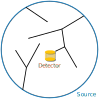
\includegraphics[width=0.66\textwidth]{chapter5/bmc_setup.pdf}
        \caption{Forward MC.}
    \end{subfigure}
    \hfill
    \begin{subfigure}[t]{0.49\textwidth}
        \centering
        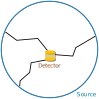
\includegraphics[width=0.66\textwidth]{chapter5/bmc_setup_backward.pdf}
        \caption{Backward MC.}
    \end{subfigure}
    \caption{
        Comparison of the forward and backward (or adjoint) configurations of
        Monte Carlo simulation, in the case where a small detector volume is
        surrounded by a comparatively large particle source. Reversing the flow
        of particle transport means that sampled events are more likely to
        contribute toward the rate estimation.
    }
    \label{fig:bmc_configuration}
\end{figure}

\subsection{Method}\label{sec:bmc_method}
% In standard Monte Carlo simulations, events are generated by a source and
% propagated forward in time according to their equations of motion and
% interaction cross-sections within any surrounding medium. In a situation where
% the source is large compared to the sensitive detector volume, as illustrated in
% Figure~\ref{fig:bmc_configuration}, events have a high probability to miss the
% % detector and contribute nothing toward the result.

In backward MC, events are generated according to an arbitrary probability
density function (PDF) around the detector volume. The overall sampling PDF is
typically the composite of a position, direction and energy sampling
distributions, i.e.\ 
\begin{align}\label{eq:sampling_pdf}
p(\bm{x}, \bm{p}, E) = p(\bm{x}) \ \times\  p(\bm{p}) \ \times\  p(E),
\end{align}
where $p$ denotes an arbitrary PDF whose integral is 1, $\bm{x}$ denotes
position, $\bm{p}$ direction and $E$ energy. If more than one particle type is
considered, the discrete distribution of particles can also enter
Equation~\ref{eq:sampling_pdf}. In our case, both atmospheric muons and anti-muons
are relevant, and they are sampled identically in equal proportions.

\sepfootnotecontent{A}{Reference~\cite{DESORGHER2010247} also provides a more
thorough discussion of adjoint cross-sections, weights, weight corrections and
source normalisation.}

Each event $i$ is propagated backward using adjoint transport and interaction
kernels such that the particle undergoes reverse energy loss and various
discrete processes, while moving backward toward the source. At each step $j$ of
the propagation, a multiplicative weight $w^i_j$ is computed given the path
taken and the interactions along it. When the particle reaches the source, the
directional flux at the source $\phi_\mathrm{s}$ is used as a normalisation
factor to yield a weighted event flux
$$
\phi(\bm{x}'_i, \bm{p}'_i, E'_i) = \prod_j w^i_j\ \times\ 
\phi_\mathrm{s}(\bm{x}'_i, \bm{p}'_i, E'_i),
$$
where $\bm{x}'$, $\bm{p}'$ and $E'$ denote respectively the position, direction
and energy of the particle upon reaching the source.

The weighted event flux $\phi$ is related to the event rate $R$ by the
inverse of the sampling PDF of Equation~\ref{eq:sampling_pdf} used to generate
the event initially:
\begin{align*}
R\,(\bm{x}_i, \bm{p}_i, E_i, \bm{x}'_i, \bm{p}'_i, E'_i) = 
    \frac{\phi_i(\bm{x}'_i, \bm{p}'_i, E'_i)}{p(\bm{x}_i, \bm{p}_i, E_i)}.
\end{align*}
Since the rate depends on the position, direction and energy of the particle at
the source, it is susceptible to variation across backward runs because of the
stochastic aspect of Monte Carlo transport. Hence, backward transport is
repeated $N$ times for each event to find the average rate
\begin{align}\label{eq:avg_rate}
\overline{R}\:(\bm{x}_i, \bm{p}_i, E_i)
    &= \sum_{k=1}^N R\,(\bm{x}_i, \bm{p}_i, E_i, \bm{x}'_k, \bm{p}'_k, E'_k) \nonumber\\
    &= \frac{1}{p(\bm{x}_i, \bm{p}_i, E_i)} \ \times\ \frac{1}{N} \sum_{k=1}^N \phi(\bm{x}'_k, \bm{p}'_k, E'_k),
\end{align}
smearing out the dependence on $\bm{x}'$, $\bm{p}'$ and $E'$. Given a large
enough $N$, i.e.\ a significant enough sample of backward transports, the sum of
weighted fluxes becomes equivalent to an integration over the possible transport paths
and interactions, and Reference~\cite{DESORGHER2010247} demonstrates that the
obtained results are consistent with forward Monte Carlo\sepfootnote{A}.



% Desorgher on the matching between forward and backward MC:
%  The Monte Carlo sampling of a big enough number of reverse tracks is
%  equivalent to the integration of the weight W over all independent variable
%  (E1,O1,Sd,x1,E0, ...) summed over all type of reverse reactions, atomic
%  elements, adjoint primaries, and adjoint secondaries. In this integration the
%  cases where more than one reaction and no reaction occur are also considered
%  and only the tracks reaching the external source are accounted for. By this
%  way the same answer is obtained as in the forward case.



% \section{ICEDUST integration}

% - New SimBackwardMC package.

% - PUMAS~\cite{pumas} as an external, with goupil stuff to handle topography,
% geomag field, etc.



\section{Application to COMET Phase-I}
% Here, talk about the COMET setup: 
% + We want to estimate the rate of background events caused by 
%   muons+secondaries hitting the detector
% + Thus, we sample muons+/- around the envelope of the CRV, according to [spell
%   out PDF]
% + We apply backward MC up to an atmospheric muon flux model at altitude X,
%   tabulated from CORSIKA etc.
% + We can first estimate the cosmic muon rate on each surface of the CRV
%   Show plots etc.
% + From the events generated at the CRV envelope, it is also possible to
%   propagate forward to determine which events might produce signal-like
%   tracks.
% + Once this is done, we use the results from backward propagation to estimate
%   rate of background-inducing cosmic muons, qed.
Backward MC simulation was used to estimate the cosmic background rate in COMET
Phase-I. This section describes the simulation setup, validations of the method
using experimental data and results of the study.

\subsection{Geometry}
The simulation geometry used in the simulation is shown in
Figure~\ref{fig:bmc_geometry}. In the COMET \mbox{Phase-I} experiment, the cosmic ray
veto (CRV) described in Section~\ref{sec:crv} will enclose the Cylindrical
Detector in order to help identify events caused by atmospheric muons. The CRV
uses a glass resistive plate chamber (GRPC) as the active detector on the
upstream-facing side, and plastic scintillator counters on the other faces. Two
holes are present in the CRV, one in the upstream face and one in the downstream
face. These holes allow atmospheric muons to sneak into the CyDet unnoticed and
potentially produce signal-like tracks, contributing to the background rate.


\begin{figure}
    \centering
    \begin{subfigure}[b]{0.56\textwidth}
        \includegraphics[width=0.95\textwidth]{chapter5/geometry.png}
        \caption{Cutaway view of the simulation world.}
    \end{subfigure}
    \hfill
    \begin{subfigure}[b]{0.41\textwidth}
        \includegraphics[width=0.95\textwidth]{chapter5/crv_geom.pdf}
        \caption{Detail of the CRV geometry.}
    \end{subfigure}
    \caption{COMET Phase-I simulation geometry used in the cosmic background study.}
    \label{fig:bmc_geometry}
\end{figure}

\subsection{Event sampling}

\subsubsection{CRV envelope sample}
As discussed in Section~\ref{sec:bmc_method}, events must be generated around
our volume of interest, the Cylindrical Detector. We define a sampling
envelope around the CRV, where muons (and anti-muons) will be generated and
backward-propagated. Events are sampled uniformly over this
envelope, i.e. the position PDF $p(\bm{x})$ is independent of $\bm{x}$:
$$
p(\bm{x}) = \frac{1}{N_{\bm{x}}},
$$
where $N_{\bm{x}}$ is the normalisation term satisfying 
$\int p(\bm{x}) \: \textnormal{d}\bm{x} = 1$.

The direction of each primary particle is sampled according to Lambert's cosine
law, which favours events with a large vertical momentum component:
$$
p(\bm{p}) = 
    \frac{1}{N_{\bm{p}}} \ (-\hat{\bm{p}}) \cdot \hat{\bm{y}} = 
    \frac{1}{N_{\bm{p}}}\:\cos(\theta_z),
$$
where $\theta_z$ is the angle between $-\bm{p}$ and the vertical axis $\hat{\bm{y}}$
(or zenith angle), and $N_{\bm{p}}$ is the normalisation factor. 

The energy of the generated muons is sampled according to an inverse law to
favour low-energy events, since they are more likely on average:
$$
p(E) = \frac{1}{N_E}  \frac{1}{E},
$$
where $N_E$ is the normalisation factor. 

The arbitrary PDFs selected for event sampling do not affect the results so long
as we ensure that no region of the phase-space which could be responsible for
backgrounds is omitted. Here, the direction and energy distributions are
optimised to favour events that are generally more likely to
occur given the configuration of our source and detector (i.e. small zenith
angles and low energies). When computing the rate for an event, any bias
originating from the sampling PDF should be cancelled out when dividing by
$p(\bm{x}, \bm{p}, E)$ as in Equation~\ref{eq:avg_rate}.



\subsubsection{CRV openings sample}
The backward MC method gives freedom to generate a specialised sample to increase
statistics in any region of phase-space. In our case, in order to focus on the
events that might sneak into the detector unnoticed by the CRV, a sample is
produced with events generated only on the holes on either side of the CRV. The
energy and direction are sampled identically to the envelope sample.

Since the position PDF in this sample is concentrated around the holes, we need
to simulate fewer events in order to find a sneaking signal-like track than with
the envelope sample. This allows us to obtain reasonable statistics in the
background rate study while saving on computational costs and storage space.



\subsection{Atmospheric muon flux}
Estimating rates requires knowledge of $\phi_s$, the directional flux at the
source. We use tabulated flux data from a CORSIKA~\cite{corsika} simulation as
an efficient way to query the flux as a function of energy and direction. The
flux data, shown as a function of energy in
Figure~\ref{fig:corsika_flux_distribution}, was estimated \SI{1600}{\metre}
above sea level for energies between \SI{10}{\MeV} and \SI{10}{\TeV}, separately
for muons and anti-muons. In the backward simulation, any event which is unable to
travel back to this infinite source plane is assumed to have a rate of zero.

\begin{figure}
    \centering
    \includegraphics[width=0.6\textwidth]{chapter5/flux_distribution.pdf}
    \caption{ Spectrum of the atmospheric muon flux (multiplied by
        $E_\mu^{2.7}$) calculated at an altitude of 1600m using a CORSIKA
        simulation. This spectrum, tabulated in both energy and zenith angle, is
        used as the flux source in the COMET Phase-I backward MC. Here, it is
        compared with the parametrisation of the muon flux at sea level from Guan
        et al.~\cite{gccly}. }
    \label{fig:corsika_flux_distribution}
\end{figure}

% Do we talk about the PUMAS, GOUPIL setup?
% ICEDUST integration?
% Maybe in appendix

% Describe data sample? How many events generated, how many times
% backward-propagated, how much storage space, etc.

\subsection{Validations}
In order to ensure that the backward MC simulation yields accurate results, the
flux of atmospheric muons estimated around the CRV is compared to two
independent measurements of the flux at sea level.

\subsubsection{BESS-TeV}
The atmospheric muon flux in Manitoba, Canada was measured using the BESS-TeV
spectrometer in 2004~\cite{besstev}. The apparatus only observed muons incident
at an near-vertical zenith angle $\theta_z$. In order to compare our simulation
results with the experimental data, we select simulated events based on the
condition that $\cos \theta_z > 0.98$ to replicate the acceptance of the
spectrometer. The comparison of the differential flux as a function of momentum
is shown in Figure~\ref{fig:bmc_validations_bess}.

\subsubsection{Kiel-DESY}
The Kiel-DESY spectrometer was used to measure the atmospheric muon flux in
Hamburg, Germany in 1975~\cite{kieldesy}. This detector measures particles
within a zenith angle $\theta_z =\SI{75}{\degree} \pm \SI{7}{\degree}$ and an
azimuthal angle $\phi = \SI{288}{\degree} \pm \SI{20}{\degree}$. Similarly to
the previous comparison, simulated events are selected to replicate these
acceptances such that the flux can be compared.
Figure~\ref{fig:bmc_validations_kiel} shows the comparison of the flux spectra.

\begin{figure}
    \centering
    \begin{subfigure}[t]{0.49\textwidth}
        \centering
        \includegraphics[width=0.95\textwidth]{chapter5/comparison_besstev.pdf}
        \caption{ Comparison to BESS-TeV spectrometer data of the atmospheric
        muon flux at a near-vertical zenith angle in Manitoba,
        Canada~\cite{besstev}. }
        \label{fig:bmc_validations_bess}
    \end{subfigure}
    \hfill
    \begin{subfigure}[t]{0.49\textwidth}
        \centering
        \includegraphics[width=0.95\textwidth]{chapter5/comparison_kieldesy.pdf}
        \caption{ 
            Comparison to the Kiel-DESY spectrometer observation of the
            atmospheric muon flux at a zenith angle of $\SI{75}{\degree} \pm
            \SI{7}{\degree}$~\cite{kieldesy} in Hamburg, Germany.}
        \label{fig:bmc_validations_kiel}
    \end{subfigure}
    \caption{ Validations of the backward MC-estimated flux with experimental
        observations of the atmospheric muon flux by two independent
        experiments. Events from the backward MC simulation are selected to
        reflect the angular acceptance of the corresponding experiment. }
    \label{fig:bmc_validations}
\end{figure}

The fact that both comparisons are in reasonable agreement with the backward
simulation results increases our confidence in the method. Here, we have shown
that the backward MC method can effectively compute the flux of events at sea
level using knowledge of the flux at an altitude of \SI{1600}{\metre}.

\subsection{Absolute rate}
From the estimated flux, one can compute the absolute rate using
Equation~\ref{eq:avg_rate}. Figure~\ref{fig:avg_rate_per_face} shows the
atmospheric muon rate as a function of momentum on each face of the CRV. The top
face is the most exposed, with an integrated rate of \SI{1.97}{\kHz}. Over the
whole surface, the estimated event rate is \SI{3.47}{\kHz}.

This estimation of the rate counts all events inbound on the CRV, regardless of
whether they enter the CDC or CTH. 


\begin{figure}
    \centering
    \includegraphics[width=0.5\textwidth]{chapter5/rate_vs_p.pdf}
    \caption{
        Average rate of inbound atmospheric muons over each face of the CRV as a
        function of momentum. Figures in parentheses in the legend are the
        integrated average rate over each face.
    }
    \label{fig:avg_rate_per_face}
\end{figure}

\subsection{$\mu$--$e$ conversion background rate}
In order to determine how many signal-like tracks are produced by atmospheric
muons, we first simulate forward the events generated around the CRV, using
\texttt{SimG4}. The events can then be selected based on detector acceptance
criteria.

\subsubsection{Track reconstruction}
We simulate the reconstruction of tracks in the CDC by fitting a helix through
the positions of hits. In this step, the true hit positions given by the
\texttt{SimG4} Monte Carlo are used. The fit returns the momentum of the
reconstructed trajectory, which is used later on to select signal-like events.

\subsubsection{Event selection}
The event selection criteria are as follows:
\begin{itemize}
    \item Fourfold coincidence: four neighbour CTH counters must be hit
    within a \SI{10}{\ns} window,
    \item CDC layers: the track must reach up to the 5th layer of CDC
    wires and no hit should occur on the outermost layer,
    \item Muon stopping target intersection: the fitted track must intersect the
    muon stopping target,
    \item Momentum window: the reconstructed momentum must lie between
    \SI{55}{\MeV/\clight} and \SI{155}{\MeV/\clight}.
\end{itemize}

\subsubsection{Backward sampling}
The flux is sampled through backward MC simulation for all events that pass the
above selection criteria. The backward propagation and flux sampling is
performed $N=5000$ times for each event. The flux for each event is the average
over these $N$ trials, as discussed in Section~\ref{sec:bmc_method}.

\subsubsection{Results}
The average rate of atmospheric muon-induced events that pass the selection
criteria is \hl{correct} \SI{100}{\Hz}. In COMET Phase-I, signal events are also
selected based on strict momentum and timing windows, as well as quality cuts.
Table~\ref{tab:bmc_bg_efficiencies} shows the efficiency factors applied to our
estimated rate to account for the Phase-I signal acceptance criteria.
Figure~\ref{fig:bmc_rate_vs_momentum} shows the estimated background event rate as a
function of the reconstructed track momentum.

\begin{table}
    \centering
    \begin{tabular}{cccccc}
        1&2&3&4&5&6\\
        1&2&3&4&5&6\\
    \end{tabular}
    \caption{Efficiency factors}
    \label{tab:bmc_bg_efficiencies}
\end{table}

\begin{figure}
    \centering
    \begin{subfigure}{0.45\textwidth}
        \centering
        %\includegraphics[width=0.6\textwidth]{}
        \caption{Without a veto.}
        \label{fig:bmc_rate_vs_momentum}
    \end{subfigure}
    \hfill
    \begin{subfigure}{0.45\textwidth}
        \centering
        %\includegraphics[width=0.6\textwidth]{}
        \caption{Including the effect of the Cosmic Ray Veto detector, assuming
        an efficiency of \SI{99.99}{\percent}.}
        \label{fig:bmc_rate_vs_momentum_crv}
    \end{subfigure}
    \caption{ $\mu$--$e$ conversion background rates from atmospheric muons
        estimated via backward MC simulation. }
\end{figure}

We also have to take into account that the CRV will identify a large fraction of
backgrounds from atmospheric muons. If we assume an identification efficiency of
\SI{99.99}{\percent}, i.e.\ one event in $10^4$ does not get vetoed by the CRV,
we obtain the background rates shown in Figure~\ref{fig:bmc_rate_vs_momentum_crv}.
Note that events sneaking in via the upstream and downstream holes of the CRV
are not affected by the CRV efficiency factor.
\chapter{COMET Phase-I Sensitivity and Background Estimates}

With the framework to simulate backgrounds from atmospheric muons in place, we
can now combine the results into a complete sensitivity and background
simulation study for COMET Phase-I. In this chapter, we discuss our simulation
samples consisting of signal, decay in orbit (DIO), and atmospheric events, and
present our resulting expectations of the performance of Phase-I.

\section{Data samples}
Three simulation samples are produced for this study. A $\mu$--$e$ conversion
sample, a DIO sample and an atmospheric muon sample. All three are simulated in
the geometrical world shown in Figure~\ref{fig:bmc_geometry}. This geometry
differs from the older TDR design~\cite{the_comet_collaboration_comet_2020} by
the number of counters in the CTH. Here, each layer of the CTH has 64 counters
instead of the original 48, which mainly affects the detector's geometrical
acceptance. In addition, the outer layer of the CTH is composed of plastic
scintillation counters rather than the originally planned Cherenkov counters. As
we shall see, this has an important effect on the detector's ability to
discriminate atmospheric anti-muons from conversion electrons.

\subsection{\texorpdfstring{$\mu$--$e$}{Muon to electron} conversion} 

\subsubsection{Sample}

The signal sample is the most straightforward to produce. We initially generate
primary electrons with energy $E=\SI{104.97}{\MeV}$ uniformly inside the
stopping target disks. Their direction is isotropically distributed, as would be
the case in the conversion process. A uniform position distribution in each disk
is not realistic, because the actual distribution depends on where in the
stopping target the muons in the beam come at rest. To account for this, the
events are weighted according to the stopping positions of muons recorded in the
MC5 simulation. The weighting factor is determined from the relative probability
for a muon to stop at the sampled position, which is estimated by histogramming
the stopping positions in each disk.
Figure~\ref{fig:stopping_position_reweighting} shows the initially-sampled
uniform position distribution, the muon stopping position distribution from MC5,
and the result of event weighting. In total, $N_\mathrm{signal} =
2\times 10^6$ events are simulated to compose the signal sample.

% After applying geom cut of CTH trigger, how many remain?

\begin{figure}
    \centering
    \begin{subfigure}[t]{0.329\textwidth}
        \centering
        \includegraphics[width=\textwidth]{chapter6/initial_conversion_position_distribution.pdf}
        \caption{Pre-weighting.}
    \end{subfigure}
    \hfill
    \begin{subfigure}[t]{0.329\textwidth}
        \centering
        \includegraphics[width=\textwidth]{chapter6/stopped_muon_distribution.pdf}
        \caption{Bound muon position distribution from MC5 used as weight.}
    \end{subfigure}
    \hfill
    \begin{subfigure}[t]{0.329\textwidth}
        \centering
        \includegraphics[width=\textwidth]{chapter6/weighted_conversion_position_distribution.pdf}
        \caption{Post-weighting.}
    \end{subfigure}
    \caption{ Initial position distribution of signal electrons before and after
        weighting them by the likelihood of a muon being bound in each bin. }
    \label{fig:stopping_position_reweighting}
\end{figure}


\subsubsection{Selection}
Signal events are selected based on detector acceptance criteria. We first
require fourfold coincidence in the CTH. Figure~\ref{fig:cydet_signal_event}
shows an example of a conversion event which passes this trigger criterion. The
fraction of events remaining defines the geometrical acceptance 
$$
A_\mathrm{geom} \equiv  \frac{\text{fourfold coincidences}}{N_\mathrm{signal}}.
$$
In this simulation, the estimated geometrical acceptance is $A_\mathrm{geom} =
\SI{21}{\percent}$. In comparison, the TDR cites $A_\mathrm{geom} =
\SI{26}{\percent}$ with the previous design of the CTH.


% Reconstruction
We do not fully simulate the reconstruction of signal electron trajectories in
the CDC. In order to approximate the effect of reconstruction uncertainties, a
smearing is applied to the true momentum of each track. The reconstructed
momentum is estimated as $p_r = p_t + x$, where $p_t$ is the true momentum of
the electron as it enters the CDC, $x \sim \mathcal{N}(0, \sigma)$, and $\sigma
= \SI{200}{\keV/\clight}$ is the expected momentum resolution of the CDC. Since
tracks are not properly reconstructed, we do not apply any track quality cuts to
select events but instead weight the signal sample by the associated efficiency
factor from Table~\ref{tab:acceptance} to account for the rejection of some events.

In this simulation sample, the initial time for each event does not correspond
to the realistic time distribution of the $\mu$--$e$ conversion process. Hence,
events are not selected based on whether they reach the detector within the
trigger time window, and we weight the sample by the trigger time window
efficiency factor instead. Similarly, the sample is weighted by the trigger and
data acquisition efficiency factors to account for the loss of acceptance from
hardware effects. Table~\ref{tab:acceptance} lists the values of these
efficiency factors.


\subsection{Muon decay in orbit}
\subsubsection{Sample}
The DIO sample is similar to the signal sample in that the initial position
of signal and DIO electrons is identically distributed. Hence, we also sample
uniformly in the stopping target disks and then weight the events according to
the MC5 stopping position distribution. Similarly, the direction of DIO
electrons is sampled isotropically. The energy distribution is thus the only
difference between the two samples. 

\begin{figure}
    \centering
    \begin{subfigure}[t]{0.4\textwidth}
    \includegraphics[width=\textwidth]{chapter6/dio_momentum_distribution_initial.pdf}
    \caption{Initial sampling.}
\end{subfigure}
    \hspace{2cm}
    \begin{subfigure}[t]{0.4\textwidth}
        \centering
        \includegraphics[width=\textwidth]{chapter6/dio_momentum_distribution_czarnecki_weighted.pdf}
        \caption{Weighted with the Czarnecki et al. parametrisation~\cite{czarnecki}.}
    \end{subfigure}
    \caption{Momentum spectrum of electrons in the DIO sample.}
    \label{fig:czarnecki_spectrum}
\end{figure}

The theoretical energy spectrum of DIO electrons produced in aluminium muonic
atoms was investigated by Czarnecki et al.~\cite{czarnecki}. Here, we use their
proposed parametrisation of the energy spectrum around the DIO energy endpoint:
\begin{equation}\label{eq:czarnecki_param}
P(E_e) = a_5 \delta^5 + a_6 \delta^6 + a_7 \delta^7 + a_8 \delta^8,
\end{equation}
where $\delta \equiv E_\mu  - E_e - \frac{E_e^2}{2 m_\mathrm{Al}}$, $E_\mu =
\SI{105.194}{\MeV}$, $m_\mathrm{Al} = \SI{25133}{\MeV}$, with the values of the
four $a$ coefficients they provide. This approximation is valid in the region
$E_e > \SI{85}{\MeV}$, which is sufficient to cover our whole DIO sample. We
use this spectrum parametrisation to weight DIO events based on their energy.
Similarly to the position weighting procedure, DIO events are first generated
with a uniform energy distribution in the range $p \in [95,
110]~\si{\MeV/\clight}$, and then weighted according to the probability for a
DIO electron to have the sampled energy. Figure~\ref{fig:czarnecki_spectrum}
shows the momentum spectrum of DIO electrons before and after weighting.

The DIO sample is composed of $N_\mathrm{DIO} = 10^7$ events in total.
Figure~\ref{fig:muon_dio_in_cydet} shows an example of a potential background
event from DIO where an electron with an energy close to the conversion energy
flies into the CyDet system and induces a trigger.

\begin{figure}
    \centering
    \includegraphics[width=0.6\textwidth]{chapter6/dio_event_in_cydet.png}
    \caption{Potential DIO-induced background with momentum $p=\SI{102}{\MeV/\clight}$.}
    \label{fig:muon_dio_in_cydet}
\end{figure}

\subsubsection{Selection}
The selection of DIO events is identical to the selection of conversion events.
We require a fourfold coincidence in the CTH, and then apply a Gaussian smear to
the true momentum of the electron to approximate track reconstruction. The same
efficiency and acceptance factors as for signal events are applied to weight the
sample and determine the absolute background contribution from the DIO process.


\subsection{Atmospheric muons}

\subsubsection{Sample}

Atmospheric muon events are simulated as discussed in
Section~\ref{sec:cosmic_event_sampling}. Two samples are produced, one around the
entire surface of the CRV and one more densely concentrated on its upstream and
downstream openings. Because of how rarely a sampled atmospheric event produces
signal-like features, the atmospheric dataset is the largest of the three, with
$1 \times 10^9$ events generated on the envelope and $1.4 \times 10^9$ on the
openings.



\begin{figure}
    \centering
    \includegraphics[width=0.6\textwidth]{chapter6/atmospheric_event_in_cydet.png}
    \caption{Cosmic ray-induced background with momentum
    $p=\SI{101}{\MeV/\clight}$. \hl{What particle type is it? What true/fitted
    momentum does it have? Where does it enter, first interact to create this
    signal-like track?}}
    \label{fig:cosmic_bg_in_cydet}
\end{figure}

\subsubsection{Selection}
As for signal and DIO events, atmospheric events must at least pass the fourfold
coincidence criterion. Unlike signal and DIO events, hit information from the
CDC is also used to select track candidates. Two criteria apply: the particle
must reach at least the 5th innermost layer of the CDC, but it should not hit
the outermost layer. Hence, we select tracks with sufficient transverse
momentum to be reconstructed, but reject tracks that either have too large a
momentum to be a signal event, or appear to enter the CDC from the outside. 

In addition, the hit positions are used to reconstruct the track using a helix
fit. The fitted trajectory should intersect the muon stopping target to pass the
selection. Figure~\ref{fig:cosmic_bg_in_cydet} shows an example of an
atmospheric event that would pass this selection. The helix fit estimates the
momentum of the particle, which is used in the analysis stage. Hence, for this
sample, we do not apply a Gaussian smear to the true momentum but use the
estimated momentum from the fit instead.

\subsubsection{Rate estimation}
As discussed in Section~\ref{sec:bmc_conversion_bg_rate}, the rate for each selected
event is estimated by backward MC simulation. The backward propagation and flux
sampling is repeated 5000 times for every event, which yields an average flux
and a statistical error shown in the results.


\subsection{Sample weighting}\label{sec:sample_weighting}
\sepfootnotecontent{fn:conv_br_norm}{The nuclear muon capture branching ratio appears in this
expression because the branching ratio of $\mu$--$e$ conversion is
conventionally normalised to $\mathcal{B}_\mathrm{capture}$.}

Because they originate from different processes, the three MC samples must be
individually weighted in order to determine the absolute contribution from each.
The conversion and DIO processes both originate from the muons bound in the
stopping target, hence we can express the total number of expected conversion
and DIO electrons in terms of the total number of stopped muons $N_\mu$.
The number of signal electrons, as a function of the conversion branching
ratio $\mathcal{B}_\mathrm{conversion}$, is:
\begin{equation}\label{eq:weight_signal}
N_\mathrm{conversion} = 
N_\mu \, \mathcal{B}_\mathrm{conversion} \, 
\mathcal{B}_\mathrm{capture} \, f_\mathrm{coherent},
\end{equation}
where $\mathcal{B}_\mathrm{capture} = 0.61$ is the branching ratio of nuclear
muon capture\sepfootnote{fn:conv_br_norm} and $f_\mathrm{coherent}=0.9$ is the
fraction of conversions that are coherent.

Similarly, the total number of DIO electrons can be expressed as:
$$
N_\mathrm{DIO} = N_\mu \, \mathcal{B}_\mathrm{DIO},
$$
where $\mathcal{B}_\mathrm{DIO} = 1 - \mathcal{B}_\mathrm{capture} = 0.39$ is
the branching ratio of DIO. Our simulation sample, however, only covers the part
of the DIO spectrum where $E_e > \SI{95}{\MeV}$, so we cannot simply use
$N_\mathrm{DIO}$ as the sample weight. The proper weight is given by 
\begin{align}\label{eq:weight_dio}
N_\mathrm{DIO}^{p>\SI{95}{\MeV}} &= N_\mathrm{DIO} \, P(E_e > \SI{95}{\MeV}) \\\nonumber
&= N_\mathrm{DIO}\,\int_{\SI{95}{\MeV}}^{E_\mathrm{endpoint}} P(E_e)\,dE_e,
\end{align}
where $E_\mathrm{endpoint} = \SI{104.973}{\MeV}$ is the energy above which no
DIO electron can be produced. The integral term in this equation is estimated by
numerically integrating the Czarnecki parametrisation of
Equation~\ref{eq:czarnecki_param}.
%  to obtain $N_\mathrm{DIO}^{p>\SI{95}{\MeV}} = 0.67$ assuming $N_\mu = 1.5e16$.

In the case of atmospheric muons, the backward MC procedure yields an absolute
rate $R$ for each event. This rate can simply be integrated over the total
data acquisition time of the experiment $T_\mathrm{DAQ}$ to obtain the expected
event count:
\begin{equation}\label{eq:weight_atmospheric}
N_\mathrm{atmospheric} = \int_0^{T_\mathrm{DAQ}} R dt = R \times T_\mathrm{DAQ}.
\end{equation}

\hl{v This is still a lie... We say otherwise two paragraphs below.}

In this study, we use the value of $T_\mathrm{DAQ} = 146$~days required for
Phase-I to reach its sensitivity goal according to the TDR. This run time
corresponds to $N_\mu = 1.5 \times 10^{16}$. In the subsequent analysis, we
substitute these two values into
Equations~\ref{eq:weight_signal},~\ref{eq:weight_dio}
and~\ref{eq:weight_atmospheric} to weight each sample.



\subsubsection{Trigger time window efficiencies}
In order to take into account the trigger timing window, we assume that
atmospheric muons irradiate the detector with a uniform time distribution.
Hence, the time window efficiency factor is the average fraction of time when
the trigger is active:
$$
\epsilon_\text{time window}^\mathrm{atmospheric} =
\frac{8}{9}\,\frac{1170 - 700}{1170} = \SI{36}{\percent}
$$
assuming the trigger window is between 700 and \SI{1170}{\ns}, and where the
factor $\frac{8}{9}$ arises from the bunch structure of the J-PARC main ring. In
contrast, the efficiency factor for conversion and DIO electrons
$\epsilon_\text{time window}^\text{conversion|DIO} = \SI{30}{\percent}$ is
smaller because the time distribution of bound muons is not uniform but peaks
around \SI{300}{\ns}, before the trigger becomes active (see
Figure~\ref{fig:timing_distributions}).



\section{Single event sensitivity}
As discussed in Section~\ref{sec:SES}, the single event sensitivity (SES) is
defined as the value of the $\mu$--$e$ conversion branching ratio required for
the experiment to observe one signal event. It can be expressed in terms of the
experimental acceptance $A_{\mu-e}$ and the total number of muons stopped in the
stopping target $N_\mu$:
\begin{equation*}
\mathrm{SES} = 
\frac{1}{N_\mu\,A_{\mu-e}\,\mathcal{B}_\mathrm{capture}\,f_\mathrm{coherent}},
\end{equation*}
where $\mathcal{B}_\mathrm{capture} = 0.61$ and $f_\mathrm{coherent} = 0.9$.

In this simulation study, we found the geometrical acceptance $A_\mathrm{geom}$
of the CyDet with the new CTH layout to be reduced from \SI{26}{\percent} to
\SI{21}{\percent}. Hence, the net signal acceptance $A_{\mu-e}$ decreases from
\SI{4.1}{\percent} to \SI{3.3}{\percent}. On the other hand, the yield of
stopped muons per proton collision was also estimated from the MC5 dataset to be
$R_{\mu / p} = 4.86 \times 10^{-4}$, which is slightly higher than the TDR value
by a factor $1.03$. Overall, although the total number of bound muons is
increased for the same run time, it is outweighed by the decrease in acceptance.
Keeping $T_\mathrm{DAQ}$ fixed at 146 days, we obtain $N_\mu = 1.53 \times
10^{16}$, hence our estimation of the COMET Phase-I sensitivity is
$$
\mathrm{SES} = 3.61 \times 10^{-15}.
$$


\section{Analysis}

After applying the efficiency factors and weighting each sample by the total
number of expected events as per Section~\ref{sec:sample_weighting}, we are able
to determine the absolute contribution from each source over a given data
acquisition period.

\subsection{Momentum spectrum} %??

\begin{figure}
    \centering
        
    \begin{subfigure}[t]{0.49\textwidth}
        \centering
        \includegraphics[width=\textwidth]{chapter6/thesis_conversion_search_momentum_distribution_nocuts_v5.pdf}
        \caption{ In the absence of event rejection by the CRV, the CTH trigger, and the timing window. }
        \label{fig:log_spectrum_nocuts}
    \end{subfigure}
    \hfill
    \begin{subfigure}[t]{0.49\textwidth}
        \centering
        \includegraphics[width=\textwidth]{chapter6/thesis_conversion_search_momentum_distribution_withcuts_except_directionID.pdf}
        \caption{ With a \SI{99.99}{\percent}-efficient CRV. 
        }
        \label{fig:log_spectrum_cuts_except_directionID}
    \end{subfigure}
    \caption{ Momentum spectrum of conversion, DIO and atmospheric events around
    the conversion energy, integrated over the Phase-I run time $T_\mathrm{DAQ}
    = 146$~days, assuming $\mathcal{B}_\mathrm{conversion} = 3.61\times
    10^{-15}$. Error bars on the atmospheric event bins show the statistical
    uncertainty from the backward MC flux estimation.
    % For atmospheric events, we compare the absence and presence of
    % the CRV in rejecting backgrounds. We also show the effect of the time
    % trigger window and track quality cuts on the signal and DIO contributions. 
    }
    \label{fig:log_spectra}
\end{figure}


The absolute event counts from conversion, DIO and atmospheric muon events are
plotted as a function of the reconstructed track momentum in
Figure~\ref{fig:log_spectra}. Note again that for conversion and DIO, $p$ is the
smeared momentum of the electron as it enters the CDC, whereas we use the
momentum reconstructed via a helix fit for atmospheric muon events.


In order to determine the effect of the CRV on the atmospheric background, as in
Figure~\ref{fig:log_spectrum_cuts_except_directionID}, we apply a weight to each
event based on whether it passed through the active material of the CRV. For
events that produce hits in the CRV, the weight is the assumed inefficiency of
the CRV, $\epsilon_\mathrm{CRV} = 1 - \SI{99.99}{\percent} = 10^{-4}$. Events
that sneak into the detector are given a weight of 1 since the CRV cannot veto
them. Similarly, to simulate the absence of the CRV, as in
Figure~\ref{fig:log_spectrum_nocuts}, all atmospheric muon events have a weight
of 1, corresponding to a \SI{0}{\percent}-efficient CRV.



\sepfootnotecontent{fn:bg_study_rmc}{ We chose not to show the RMC spectrum in
    our plots because the contribution from RMC is smaller than that of DIO by a
    factor of 5~\cite{the_comet_collaboration_comet_2020}.}



% However, by investigating where
% these background events come from, we will see that there are ways to identify
% some of them and reduce their contribution below the single-event threshold.

The reconstructed momentum of the candidate track is one of the most important
criteria in discriminating signal electrons from DIO or
RMC\sepfootnote{fn:bg_study_rmc} electrons, because the energy spectra of the
latter two fall off sharply close to the conversion energy. In Phase-I, the
momentum window within which an event is counted is $p \in [103.6,
106.0]\,\si{\MeV/\clight}$. This cut eliminates the overwhelming majority of DIO
and RMC backgrounds. However, atmospheric background events appear to be uniformly
distributed in this region, making the cut ineffective in rejecting them. 

Figure~\ref{fig:log_spectrum_nocuts} shows that in the absence of the CRV,
atmospheric backgrounds overwhelm the detector and outnumber conversion events
by three orders of magnitude in the momentum window. In the presence of the CRV,
and assuming an efficiency of \SI{99.99}{\percent}
(Figure~\ref{fig:log_spectrum_cuts_except_directionID}), atmospheric backgrounds
are suppressed by a factor $10^3$. However, their integrated count still exceeds
one, making the $\mu$--$e$ conversion search impossible unless there is an
additional way to identify them.


% This is like a hard conclusion to swallow, should go at the end of the section
% so we can move straight to the ways in which we can try to identify atmos.


% For the atmospheric sample, we also reduce the background rate of certain events
% based on the primary particle ($\mu^-$ or $\mu^+$) and whether they hit the CRV.
% The first stage of the CTH, containing only scintillation counters and no
% Cherenkov counters, is unable to differentiate muons from electrons. Hence,
% signal-like tracks induced by sneaking atmospheric $\mu^+$ are a major source of
% backgrounds in this situation. 






\subsection{Particle identification}
%\subsection{Atmospheric \texorpdfstring{$\mu^+$}{anti-muon} backgrounds and particle identification}

In Figure~\ref{fig:log_spectrum_cuts_except_directionID}, we assumed that the
CyDet has no way of discriminating between electrons, muons, and anti-muons.
This is partly true since the first stage of the CTH will be composed of only
scintillation counters. These cannot help to identify the particle type like
Cherenkov counters, which are planned to replace one layer of scintillators in
the second stage of the CTH.

We investigate the effect of direction identification and CRV efficiency on the
background rate.

Positive muons can produce signal-like tracks in the CyDet by following the
reverse path of a conversion electron. Why? I have to explain exactly why.
Candidate signal electron trajectories originate in the muon stopping target,
produce a helical track in the CDC, and induce a fourfold coincidence in the
CTH. A $\mu^+$ can generate a background event by first hitting the CTH,
producing a track in the CDC, and then intersecting the muon stopping target,
appearing as a conversion track in reverse time ordering.

Question: if a mu+ follows the same time ordering as an e-, what does it look
like in the CyDet? 1. It curves in the other way as a negative particle in the B
field. Can that be easily rejected by the detector? At which step?

Paragraph: the stage-1 CTH can't do PID. Explain why, using Cherenkov counter
properties vs plastic scintillator.

Paragraph: reverse-direction mu+ track can still be identified via
time-of-flight information. Method was investigated internally by Moritsu, who
determined that direction identification method can reject 89 percent of
atmospheric mu+ events with, but reduces the net signal acceptance by a
factor 0.87.



\subsection{CRV efficiency}

\begin{figure}
    \centering
    \includegraphics[width=0.5\textwidth]{chapter6/bg_count_vs_crv_efficiency.pdf}
    \caption{ Integrated atmospheric background count as a function of the CRV
        efficiency. The lower bound arises from sneaking events which cannot be
        identified by the CRV. More accurate particle identification by the
        CyDet helps to reduce this sneaking component, e.g.\ by discriminating
        muons from electrons.}
    \label{fig:bg_count_vs_crv_efficiency}
\end{figure}

The CRV efficiency determines the fraction of atmospheric events which
can enter the CyDet through the active parts of the CRV while not being vetoed.
Although we have assumed so far that the CRV is \SI{99.99}{\percent}
efficient, it will not necessarily be the case in practice.

Note that the portion of background events produced by atmospheric muons
sneaking through the CRV openings is unaffected by how efficient the CRV is.
These backgrounds can only be reduced by increasing the coverage of the CRV,
which has inherent limitations since the beam must enter on one side and exit
on the other.


\chapter{Conclusion}

% Muon and LFV
Since the discovery of the muon in 1937, our understanding of its properties has
been steadily evolving. Today, although it fits nicely into the Standard Model
of particle physics, some questions remain standing, and recent tensions
observed between theory and experiment are suggesting that the SM does not give
a complete picture of the muon's underlying nature. Charged lepton flavour
violation is one of the ways in which Nature might deviate from the SM. If CLFV
were observed, it would be a clear indication of new physics. Neutrino-less
muon-to-electron conversion is one of the most sensitive channels to search for
CLFV as its signature is a mono-energetic electron with few sources of potential
backgrounds. According to theoretical constraints, this process ought to be
suppressed beyond experimental sensitivities. Therefore, any observation of the
$\mu$--$e$ conversion signal would yield clear evidence for CLFV and hence guide
the field toward a better understanding of physics beyond the Standard Model.

% COMET
The COMET Phase\nobreakdash-I experiment will soon start its data acquisition run toward the
search for muon-to-electron conversion in aluminium. It is expected to be a
hundred times more sensitive to $\mu$--$e$ conversion than the previous best
measurement by SINDRUM II. To achieve this sensitivity, COMET Phase\nobreakdash-I will
produce an intense pulsed muon beam directed toward an aluminium target to
create muonic aluminium atoms, from which conversion electrons may emerge. The
Cylindrical Detector, which surrounds the muon stopping target, is designed to
clearly identify conversion electrons while rejecting as many experimental
backgrounds as possible. 

% Software & sim
In order to cover the needs of the experiment in terms of simulation,
calibration, reconstruction, data formats and data analysis, the COMET
collaboration develops a comprehensive set of software utilities named ICEDUST.
The work presented throughout this thesis relies heavily on Monte Carlo (MC) data
produced by ICEDUST's {\sc Geant4} simulations of Phase\nobreakdash-I.
% Here is a good place to kind of introduce the problem of producing large-scale
% datasets and estimating atmospheric backgrounds
MC simulations allow us to study the experiment outcomes and to optimise its
design before assembly. However, they are computationally expensive and
typically only allow us to simulate a small fraction of the amount of data
expected to be collected. Additionally, traditional MC sampling is particularly
inefficient when the source of events is far from the detector system, as is the
case when considering cosmic ray-induced backgrounds. This thesis aims to
address these two limitations by partially circumventing the brute force MC
method.

% GAN
We investigate a novel approach to the mass-production of simulation data based
on Generative Adversarial Networks. We propose a neural network generator of
hits for the Cylindrical Drift Chamber, which can produce synthetic energy
deposits in the detector at a rate $10^6$ times higher than the ICEDUST
simulation. The machine learning model is trained on a sample of simulated hits
and learns from their features and relationships. The trained model allows us to
generate only a subset of the hits produced by MC simulation, but far more
efficiently than was previously achievable. Our ambition for this work and
future developments is to enable the production of entire mock datasets, which
can be used by the collaboration in anticipation of data acquisition runs.

% BMC & background study
Additionally, we present a study of the backgrounds caused by cosmic ray-induced
atmospheric muons in the COMET Phase\nobreakdash-I muon-to-electron conversion search. We
use a backward Monte Carlo simulation method to efficiently estimate the flux of
atmospheric muons near the detector system. We then perform a full analysis of
the event count contributions from $\mu$--$e$ conversion, muon decay-in-orbit,
and atmospheric muons. Our findings suggest that an efficient rejection of
atmospheric backgrounds by the Cosmic Ray Veto, combined with particle-type
identification by the Cylindrical Detector, are necessary for the Phase\nobreakdash-I search
to succeed. Under optimistic conditions, namely with a
\SI{99.99}{\percent}-efficient CRV and \SI{99}{\percent} muon identification
rate by the CyDet, we expect 0.08 atmospheric background events during the 146
days of data acquisition. According to our analysis, during this run time, COMET
Phase\nobreakdash-I will be able to achieve a single event sensitivity of $3.61 \times
10^{-15}$.


% Wrap up: what do my results mean for COMET!!!
Our most important contributions have been integrated into the main ICEDUST
software repository and documented for others to use and build upon. As the
COMET experiment goes into the Phase\nobreakdash-I measurement period, we hope that these
techniques will help to refine our understanding of the data and that they can
be applied in preparation for Phase\nobreakdash-II and beyond.

\appendix
\chapter{Appendix A}

\printbibliography

\listoffigures
\listoftables

\end{document}
